\documentclass[lang=cn,11pt]{elegantbook}
\usepackage[utf8]{inputenc}
\usepackage[UTF8]{ctex}
\usepackage{amsmath}%
\usepackage{amssymb}%
\usepackage{graphicx}
\usepackage{pdfpages}
\usepackage{algorithm}
\usepackage{algpseudocode}

\title{CSE 545: Machine Learning}
\subtitle{25 Win, instructed by Honglak Lee}

\begin{document}
\frontmatter
\tableofcontents
\mainmatter

\chapter{on Linear Regression}
\section{Derivation and Proof}

\subsection{Derive the solution for \(w_0\) and \(w_1\) in linear regression}
Consider the linear regression problem for 1D data, where we would like to learn a function \(h(x) = w_1x + w_0\) with parameters \(w_0\) and \(w_1\) to minimize the sum squared error:

\[
L = \frac{1}{2} \sum_{i=1}^{N} (y^{(i)} - h(x^{(i)}))^2
\]

for \(N\) pairs of data samples \((x^{(i)}, y^{(i)})\). Derive the solution for \(w_0\) and \(w_1\) for this 1D case of linear regression. Show the derivation to get the solution:

\[
w_0 = Y - w_1X,
\]

\[
w_1 = \frac{\frac{1}{N} \sum_{i=1}^{N} x^{(i)} y^{(i)} - YX}{\frac{1}{N} \sum_{i=1}^{N} (x^{(i)})^2 - X^2},
\]

where \(X\) is the mean of \(\{x^{(1)}, x^{(2)}, \ldots, x^{(N)}\}\) and \(Y\) is the mean of \(\{y^{(1)}, y^{(2)}, \ldots, y^{(N)}\}\).

\begin{proof}
(As we know, this is a convex function of $w$ and the critical point for a convex function is a global min. So we )
We first derive the optimal for $w_0$:
\[
\frac{\partial L}{\partial w_0}
= \frac{\partial}{\partial w_0}
   \Bigl[
       \tfrac{1}{2}\sum_{i=1}^N \bigl(y^{(i)} - w_1 x^{(i)} - w_0\bigr)^2
   \Bigr]
\]
For each \(i\), we have (by chain rule)

\[
\frac{\partial}{\partial w_0}
\bigl(y^{(i)} - w_1 x^{(i)} - w_0\bigr)^2
= 2\,\bigl(y^{(i)} - w_1 x^{(i)} - w_0\bigr)\,(-1)
\]
Setting the partial to 0:
\begin{align}
    \frac{\partial L}{\partial w_0}
&= -\sum_{i=1}^N \bigl[y^{(i)} - (w_1 x^{(i)} + w_0)\bigr] = 0 \\
\sum_{i=1}^N y^{(i)} 
&= \sum_{i=1}^N \bigl(w_1 x^{(i)} + w_0\bigr)\\
& = w_1 \sum_{i=1}^N x^{(i)} + N\,w_0
\end{align}
Then dividing by $1/N$ in both sides:
\begin{align}
    \frac{1}{N}\sum_{i=1}^N y^{(i)} 
&= w_1 (\frac{1}{N}\sum_{i=1}^N x^{(i)}) + w_0 \\
\overline{Y} &=     w_1   \overline{X} + w_0
\end{align}
Thus we have 

\[
w_0 = \overline{Y} - w_1 \, \overline{X}
\tag{1}
\]
Next, we derive the optimal value of $w_1$.
\[
\frac{\partial L}{\partial w_1}
= \frac{\partial}{\partial w_1}
   \Bigl[
       \tfrac{1}{2}\sum_{i=1}^N \bigl(y^{(i)} - w_1 x^{(i)} - w_0\bigr)^2
   \Bigr].
\]
for each \(i\), we have (by chain rule):
\[
\frac{\partial}{\partial w_1}
\bigl(y^{(i)} - w_1 x^{(i)} - w_0\bigr)^2
= 2\,\bigl(y^{(i)} - w_1 x^{(i)} - w_0\bigr)\,(-\,x^{(i)}).
\]

So by setting the partial to 0:
\begin{align}
    \frac{\partial L}{\partial w_1}
= -\sum_{i=1}^N 
    \bigl[y^{(i)} - (w_1 x^{(i)} + w_0)\bigr] \, x^{(i)} &= 0\\
\sum_{i=1}^N y^{(i)} x^{(i)}
&= \sum_{i=1}^N (w_1 x^{(i)} + w_0)\, x^{(i)} \\
\sum_{i=1}^N y^{(i)} x^{(i)}
&= w_1 \sum_{i=1}^N (x^{(i)})^2 
  \;+\; w_0 \sum_{i=1}^N x^{(i)}
\end{align}
Using (1) for $w_0$, and dividing by $1/N$ on both sides:
\begin{align}
\frac{1}{N}\sum_{i=1}^N x^{(i)} y^{(i)}
& = w_1 \,\frac{1}{N}\sum_{i=1}^N (x^{(i)})^2 
  \;+\; (\overline{Y} - w_1 \overline{X})\overline{X} \\
&=  w_1 \left[\frac{1}{N}\sum_{i=1}^N (x^{(i)})^2 - X^2\right]
  + \overline{Y} \overline{X}
\end{align}
Resolving for \(w_1\):
\[
w_1 
= \frac{
   \frac{1}{N}\sum_{i=1}^N x^{(i)} y^{(i)} - \overline{X} \overline{Y}
}{
   \frac{1}{N}\sum_{i=1}^N (x^{(i)})^2 - \overline{X}^2
}
\tag{2}
\]
This completes the solution for both $w_0$ and $w_1$.
\end{proof}

\subsection{positive definite matrices}
Recall the definition and property of positive (semi-)definite matrix. Let \(A\) be a real, symmetric \(d \times d\) matrix. \(A\) is positive semi-definite (PSD) if, for all \(z \in \mathbb{R}^d\), \(z^\top A z \geq 0\). \(A\) is positive definite (PD) if, for all \(z \neq 0\), \(z^\top A z > 0\). We write \(A \succeq 0\) when \(A\) is PSD, and \(A \succ 0\) when \(A\) is PD.

It is known that every real symmetric matrix \(A\) can be factorized via the eigenvalue decomposition:
\(A = U \Lambda U^\top\), where \(U\) is a \(d \times d\) matrix such that \(UU^\top = U^\top U = I\) and \(\Lambda = \text{diag}(\lambda_1, \lambda_2, \ldots, \lambda_d)\). Multiplying on the right by \(U\), we see that \(AU = U \Lambda\). If we let \(u_i\) denote the \(i\)-th column of \(U\), we have \(Au_i = \lambda_i u_i\) for each \(i\); \(\lambda_i\) are eigenvalues of \(A\), and the corresponding columns of \(U\) are eigenvectors associated with \(\lambda_i\). The eigenvalues constitute the "spectrum" of \(A\).

\begin{enumerate}
    \item[i]. Prove \(A\) is PD if and only if \(\lambda_i > 0\) for each \(i\). (Note: "if and only if" means proving both directions.)
\begin{proof}
Let \(A\) be a real \(d\times d\), symmetric matrix, with eigen-decomposition
\[
A = U\Lambda U^\top
\]
where \(U\) is an orthogonal matrix and \(\Lambda = \mathrm{diag}(\lambda_1,\lambda_2,\dots,\lambda_d)\) is a diagonal matrix of the eigenvalues.

\textbf{forward direction \(\Rightarrow\):}  Assume \(A\) is positive definite. Let \(u_i\) be an eigenvector of \(A\) with eigenvalue \(\lambda_i\). Then \[
   u_i^\top A\,u_i 
   = u_i^\top \,\bigl(\lambda_i u_i\bigr) 
   = \lambda_i\,u_i^\top u_i
   = \lambda_i\,\|u_i\|^2 >  0
\]
Since \(u_i\neq 0\), must have \(\|u_i\|^2 > 0\), and therefore \(\lambda_i > 0\). This holds for each $i$, so all eigenvalues are positive.

\textbf{backward direction (\(\Leftarrow\)):} Conversely, assume \(\lambda_i > 0\) for every \(i\).  Let $z \not = 0 \in \mathbb{R}^d$ be arbitrary vector, then \[
   z^\top A\,z 
   = z^\top (U\,\Lambda\,U^\top)\,z 
   = (U^\top z)^\top \Lambda \,(U^\top z)
   \]
   Let \(w = U^\top z\). Note that \(w \neq 0\) whenever \(z \neq 0\) (since \(U\) is invertible). Then: \[
   z^\top A\,z 
   = w^\top \Lambda\,w 
   = \sum_{i=1}^d \lambda_i\, w_i^2.
   \]Since \(\lambda_i > 0\) and at least one \(w_i^2 \ge 0\) (since \(w\neq 0\)), we get  \(\sum_{i=1}^d \lambda_i w_i^2 > 0.\)\\
Therefore \(z^\top A\,z > 0\). Since $z$ is arbitrary, finishing the proof that \(A \succ 0\).\\
Thus, \(A\succ 0\) \(\Longleftrightarrow\) all eigenvalues \(\lambda_i>0\).\\\\
\end{proof}


    \item[ii]  Consider the linear regression problem where \(\Phi\) and \(y\) are as defined in class. The closed-form solution becomes \((\Phi^\top \Phi)^{-1} \Phi^\top y\). \\
    Now consider a ridge regression problem with the regularization term \(\frac{1}{2\beta}\|w\|_2^2\). The symmetric matrix in the closed-form solution is \(\Phi^\top \Phi + \beta I\). Derive the eigenvalues and eigenvectors for \(\Phi^\top \Phi + \beta I\) with respect to the eigenvalues and eigenvectors of \(\Phi^\top \Phi\), denoted as \(\lambda_i\) and \(u_i\). Prove that the matrix \((\Phi^\top \Phi + \beta I)\) is PD for any \(\beta > 0\).
\begin{proof}
(1) Eigenvalues/eigenvectors of \(\Phi^\top \Phi + \beta I\): 
Since $\Phi^T\Phi$ is real symmetric, suppose \(\Phi^\top \Phi\) eigen-decomposes as:\[
   \Phi^\top \Phi = U\,\Lambda\,U^\top
   \]Then \[
   \Phi^\top \Phi + \beta I 
   = U\,\Lambda\,U^\top + \beta\,I
   \]
We can rewrite \(
   \beta\,I 
   = \beta\,U\,U^\top
   \)since \(U\,U^\top = I\). Hence, \[
   \Phi^\top \Phi + \beta I 
   = U\,\Lambda\,U^\top + \beta\,U\,U^\top
   = U\,(\Lambda + \beta I)\,U^\top.
   \]
Thus the eigenvectors of \(\Phi^\top \Phi + \beta I\) are the same as those of \(\Phi^\top \Phi\) (the columns of \(U\)), and the eigenvalues are \(\lambda_i + \beta\).

(2) Positivity of \(\Phi^\top \Phi + \beta I\):  \\
\textbf{Claim: for any matrix $A$, $A^T A$ is potisive semidefinite.}\\
\noindent Proof of claim: let $x$ be arbitary  nonzero input to $A^TA$, then
$$x^T(A^TA)x=(Ax)^T(Ax)=||Ax||_2≥0$$
Therefore \(\Phi^\top \Phi\) is positive semidefinite, so its eigenvalues \(\lambda_i \ge 0\) (for the same reasoning as the proof in in(i).) Adding \(\beta I\) shifts each eigenvalue by \(\beta > 0\). Hence each eigenvalue of \(\Phi^\top \Phi + \beta I\) is \(\lambda_i + \beta > 0\). Therefore, \(\Phi^\top \Phi + \beta I\) is positive definite for any \(\beta > 0\), by (i).
\end{proof}

\end{enumerate}



\subsection{Maximizing log-likelihood in logistic regression}
In this sub-problem, logistic regression is used to predict the class label \(y \in \{-1, +1\}\) instead of \(y \in \{0, 1\}\). Show that maximizing the log-likelihood of logistic regression,

\[
\sum_{n=1}^{N} \log P(y^{(n)}|x^{(n)}),
\]

is equivalent to minimizing the following loss function:

\[
\sum_{n=1}^{N} \log \left( 1 + \exp(-y^{(n)} \cdot w^\top \phi(x^{(n)})) \right).
\]
[Hint: You can expand the log-likelihood as follows: 
\[
log P(y^{(n)} | x^{(n)}) = I(y^{(n)} = 1) log P(y^{(n)} = 1 | x^{(n)}) + I(y^{(n)} = -1) log P(y^{(n)} = -1 | x^{(n)})
\]
and then plug in the class posterior probability of the logistic regression model.]
\begin{proof}
The log-likelihood for data \(\{(x^{(n)}, y^{(n)})\}_{n=1}^N\) is
\[
\log \prod_{n=1}^N P\bigl(y^{(n)} \mid x^{(n)}\bigr)
\;=\;
\sum_{n=1}^N \log P\bigl(y^{(n)} \mid x^{(n)}\bigr)
\]
Since 
\[
P(y=+1 \mid x) 
= \sigma\bigl(w^\top \phi(x)\bigr)
\]
\[
P(y=-1 \mid x) 
= 1 - \sigma\bigl(w^\top \phi(x)\bigr)
\]
and $\sigma(-a) = 1 - \sigma(a)$, so we can write:
\[
P\bigl(y^{(n)} \mid x^{(n)}\bigr)
= \sigma\bigl(y^{(n)}\,w^\top \phi(x^{(n)})\bigr)
\]
Hence the log-likelihood is:
\[
\sum_{n=1}^N \log \sigma\bigl(y^{(n)}\,w^\top \phi(x^{(n)})\bigr)
\]
Since \(\sigma(z) = 1 / [1 + \exp(-z)]\), \(
\log \sigma(z)
= -\log\bigl(1 + \exp(-z)\bigr)
\), we have 
\[
\log \sigma\bigl(y^{(n)}\,w^\top \phi(x^{(n)})\bigr)
= -\log\bigl[1 + \exp\bigl(-\,y^{(n)}\,w^\top \phi(x^{(n)})\bigr)\bigr]
\]
Thus,
\[
\sum_{n=1}^N \log P\bigl(y^{(n)}\mid x^{(n)}\bigr)
= \sum_{n=1}^N \log \sigma\bigl(y^{(n)}\,w^\top \phi(x^{(n)})\bigr)
= -\sum_{n=1}^N \log\Bigl[1 + \exp\bigl(-\,y^{(n)}\,w^\top \phi(x^{(n)})\bigr)\Bigr]
\]
This finishes the proof that 
\[\text{maximizing}
\sum_{n=1}^N \log P\bigl(y^{(n)}\mid x^{(n)}\bigr)
\Longleftrightarrow
\text{minimizing}
\sum_{n=1}^N \log\Bigl[1 + \exp\bigl(-\,y^{(n)}\,w^\top \phi(x^{(n)})\bigr)\Bigr].
\]
\end{proof}


\section{Linear Regression on a Polynomial}
In this problem, you will implement linear regression on a polynomial. Please have a look at the accompanied starter code linear regression.py and notebook linear regression.ipynb for instructions first. Please note that all the sub-questions without (Autograder) need to be answered in your writeup.

\textbf{Sample data}: The files `q2xTrain.npy`, `q2xTest.npy`, `q2yTrain.npy` and `q2yTest.npy` specify a linear regression problem for a polynomial. `q2xTrain.npy` represent the inputs $(x^{(i)} ∈ \mathbb{R})$ and `q2yTrain.npy` represents the outputs $(y^{(i)} ∈ \mathbb{R})$ of the training set, with one training example per row.

\subsection{GD and SGD}
You will compare the following two optimization methods, in finding the coefficients of a polynomial of degree one (i.e. slope and intercept) that minimize the training loss.
• Batch gradient descent (GD)
• Stochastic gradient descent (SGD)
Here, as we seen in the class, the training objective is defined as:
$$
E(w) = \frac{1}{2} \sum_{i=1}^N (\sum_{j=0}^{M-1}w_j \phi(x^{(i)})- y^{(i)})^2  = \frac{1}{2} (w^T\phi(x^{(i)}) - y^{(i)})^2
$$
\noindent \textbf{(a) }\textbf{[12 points] (Autograder)} Implement the GD and SGD optimization methods. For all the implementation details (e.g., function signature, initialization of weight vectors, etc.), follow the instruction given in the code files. Your score for this question will be graded by the correctness of the implementation.\\
\noindent \textbf{(b) }\textbf{[3 points]} Please share the plot generated from the section 2(b) of your .ipynb file in your write-up, and then compare two optimization methods, GD and SGD. Which one takes less time and which one shows lower test objective $E(w_{test})$?
\begin{solution}
\pic[0.6]{assets/1(2b).png}
"GD version took 0.00 seconds\\
GD Test objective = 2.7017\\
SGD version took 0.06 seconds\\
SGD Test objective = 2.6796"\\
In our example, GD takes shorter time than SGD. One reason it that we have extremely small scale of 20 data points, so we can make full use of parallel computing. Through vectorization, for the 200 epoches, we takes about 200 computation. But for SGD, we iterate through the whole data set every time, so we takes about 200*20 = 4000 computations. But for larger sample scale and more schochastic choice of data points each epoch (instead of going through the whole dataset), SDG could take shorter time.\\
SGD performs a little bit better on test objective than GD. It could help escape local minima and more possibly lead to better global solution.
\end{solution}

\subsection{Over-fitting Study}
Next, you will investigate the problem of over-fitting. Recall the figure from lecture that explored over-fitting as a function of the number of features (e.g., \( M \), the number of terms in a \((M - 1)\)-degree polynomial). To evaluate this behavior, we examine the Root-Mean-Square (RMS) Error defined below. (Note: we use the RMS error just for evaluation purposes, NOT as a training objective.)

\[
E_{\text{RMS}} = \sqrt{\frac{2E(w^*)}{N}}
\]
\pic[0.6]{assets/1(2.2).png}


\noindent \textbf{(a) [8 points] (Autograder)} Implement the closed-form solution of linear regression (assuming all conditions are met) instead of iterative optimization methods. (Hint: we recommend using \texttt{np.linalg.inv} to compute the inverse of a matrix.)\\
\textbf{(b) [2 points]} Regenerate the plot with the provided data. The sample training data can be generated with \((M - 1)\)-degree polynomial features (for \( M = 1, 2, \dots, 10 \)) from \texttt{q2xTrain.npy} and \texttt{q2yTrain.npy}. We assume the feature vector is:

\[
\phi(x^{(i)}) = (1, x^{(i)}, (x^{(i)})^2, \dots, (x^{(i)})^{M-1})
\]

for any value of \( M \). For the test curve, use the data in \texttt{q2xTest.npy} and \texttt{q2yTest.npy}. Note that the trend of your curve is not necessarily the same as the sample plot. Attach your plot to the \textbf{write-up}.
\begin{solution}
\pic[0.6]{assets/1(2d).png}
\end{solution}


\textbf{(c) [2 points]} In the \textbf{write-up}, discuss: Which degree polynomial would you say best fits the data? Was there evidence of under/over-fitting the data? Use your generated plots to justify your answer.
\begin{solution}
As $M$ become larger, the training and testing $E_{RMS}$ both went down before $M = 6$, stayed still for $M=6$ through $M=8$, and after $M$ went beyong $8$, the training $E_{RMS}$ kept on going down, but the testing $E_{RMS}$ suddenly went up. This is probably the point where over-fitting began.\\
    I would say $M=6$, i.e. the $5$ degree polynomial best fits the data. This is because $M=6$ reaches both the lowest training and testing $E_{RMS}$.
\end{solution}


\subsection{Regularization (Ridge Regression)}
Finally, you will explore the role of regularization. Recall the image from lecture that explored the effect of the regularization factor \( \lambda \).
\pic[0.6]{assets/1(2.3).png}

\textbf{(a) [8 points] (Autograder)} Implement the closed-form solution of ridge regression. Specifically, use the following regularized objective function:
\[
\frac{1}{2} \sum_{i=1}^N (w^\top \phi(x^{(i)}) - y^{(i)})^2 + \frac{\lambda}{2} \|w\|_2^2
\]
to optimize the parameters \( w \).\\

\textbf{(b) [2 points]} For the sample data, regenerate the plot (Figure 2) with \( \lambda \in \{10^{-5}, 10^{-4}, \dots, 10^{-1}, 10^0 (= 1)\} \). First, compute the \( E_{\text{RMS}} \) over the training data specified in \texttt{q2xTrain.npy} and \texttt{q2yTrain.npy} with \( \lambda \), and then measure the test error using \texttt{q2xTest.npy} and \texttt{q2yTest.npy}. Attach your (unregularized) \( E_{\text{RMS}} \) plot of both the training and test data obtained from 2(g) to the \textbf{write-up}. Note that the trend of your curve is not necessarily the same as the sample plot.
\pic[0.6]{assets/1(2g).png}

\textbf{(c) [2 points]} Discuss: Which \( \lambda \) value seemed to work best for a ninth-degree polynomial (\( M = 10 \))? Use your generated plots to justify your answer. Provide your answer in the \textbf{write-up}.
\begin{solution}
    I think $\lambda = 0.0001$, i.e. $\log_{10} \lambda = -4$ seemed to work best for a ninth-degree polynomial. As shown in the plot, when fixing $M=10$,  $\log_{10} \lambda = -4$ has the lowest testing error, and the training error is stable around the point. It shows that this regularization coefficient both can prevent over-fitting and keep descent expressibility of the model.
\end{solution}



\section{Locally Weighted Linear Regression}

Consider a linear regression problem in which we want to weight different training examples differently. Specifically, suppose we want to minimize:

\[
E_D(w) = \frac{1}{2} \sum_{i=1}^N r^{(i)}(w^\top x^{(i)} - y^{(i)})^2,
\]

where \( r^{(i)} \in \mathbb{R} \) is the “local” weight for the sample \( (x^{(i)}, y^{(i)}) \). In class, we worked on a special case where all the weights \( r^{(i)} \) are equal. In this problem, we generalize these ideas to the weighted setting and implement the locally weighted linear regression algorithm.

\textbf{Notes:}
1. The weight \( r^{(i)} \) can be different for each of the data points in the training data.
2. For a 1-dimensional input \( x \) (provided in this problem), the model can be written as \( w_0 + w_1x \), where \( w_0 \) acts as the intercept term. This is naturally incorporated by extending \( x \) to include a constant term, such as \( x = [1, x]^\top \), in the formulation of the linear model.

\textbf{(a) [3 points]} Show that \( E_D(w) \) can also be written as:

\[
E_D(w) = (w^\top X - y^\top)R(w^\top X - y^\top)^\top,
\]

for an appropriate diagonal matrix \( R \), where \( X \in \mathbb{R}^{D \times N} \) is a matrix whose \( i \)-th column is \( x^{(i)} \in \mathbb{R}^{D \times 1} \), and \( y \in \mathbb{R}^{N \times 1} \) is the vector whose \( i \)-th entry is \( y^{(i)} \). Here, in locally weighted linear regression, we use raw data directly without mapping to high-dimensional features (i.e., each input is represented as a \( D \)-dimensional input vector, not an \( M \)-dimensional feature vector). Hence, we use the notation \( X \) instead of \( \Phi \). Clearly state what the \( R \) matrix is.
\begin{proof}
    
\textbf{Let \( R_0 \in \mathbb{R}^{N \times N} \) be the diagonal matrix with \( r^{(i)} \) as the \( i \)-th diagonal element.}
Note that the residual vector is:
\[
(w^\top X - y^\top)^\top = X^\top w - y
\]
Then we have:
$$
R_0(X^\top w - y) =  \begin{bmatrix} r^{(1)}(w^\top x^{(1)} - y^{(1)}) \\ \cdots \\r^{(N)}(w^\top x^{(N)} - y^{(N)})
\\ \end{bmatrix}
$$
Therefore the error function is:
\begin{align*}
  E_D(w) &= \frac{1}{2} \sum_{i=1}^N r^{(i)}(w^\top x^{(i)} - y^{(i)})^2 \\
  &= 
\frac{1}{2}\begin{bmatrix} (w^\top x^{(1)} - y^{(1)}) \\ \cdots \\(w^\top x^{(N)} - y^{(N)})
\\ \end{bmatrix}^T \begin{bmatrix} r^{(1)}(w^\top x^{(1)} - y^{(1)}) \\ \cdots \\r^{(N)}(w^\top x^{(N)} - y^{(N)})
\\ \end{bmatrix} \\
&=  \frac{1}{2}(X^\top w - y)^T (R_0(X^\top w - y))\\
&= \frac{1}{2}(w^\top X - y^\top) R_0 (w^\top X - y^\top)^T
\end{align*}
We let $R := \frac{1}{2} R_0$, then we have 
$$
E_D(w) = (w^\top X - y^\top) R (w^\top X - y^\top)^T
$$

\end{proof}

\textbf{(b) [7 points]} If all \( r^{(i)} \)'s equal 1, the normal equation for \( w \in \mathbb{R}^{D \times 1} \) becomes:

\[
XX^\top w = Xy,
\]

and the value of \( w^* \) that minimizes \( E_D(w) \) is given by:

\[
w^* = (XX^\top)^{-1}Xy.
\]

Now, by finding the derivative \( \nabla_w E_D(w) \) from part (a) and setting it to zero, generalize the normal equation and the closed-form solution to the locally weighted setting. Provide the new value of \( w^* \) that minimizes \( E_D(w) \) in a closed form as a function of \( X \), \( R \), and \( y \). (Hint: \( \nabla_w (RX^\top w) = XR^\top = XR \).)
\begin{solution}

    Define $$
    z := X^Tw - y
    $$
    Notice we have:
    $$
   z =  (w^\top X - y^\top)^\top 
    $$
And we define $F(z):= z^T R z$, then we have $E(w) = F(z)$.\\
Here we denote the derivative of a function: $f:\mathbb{R}^n \rightarrow \mathbb{R}^m$ by $D(f)$. \\
By chain rule of differentiation:
\begin{align}
D(E(w)) &= D(F(z)) D(z(w))      \\
& = D_z(z^T Rz) D_w(X^T w  - y) \\
&= (2Rz)^T X^T \\
&= (2XRz)^T
\end{align}
Thus
$$
\nabla E(w) = D(E(w))^T = 2XRz = 2XR(X^T w - y)
$$

Then setting $ \nabla E(u)= 0$, we have $2XRX^T w =  XRy$, so 
$$w_{*} = \frac{1}{2}(XRX^T)^{-1} XRy$$
This is the solution.
\end{solution}


\textbf{(c) [8 points]} Suppose we have a training set \( \{(x^{(i)}, y^{(i)}); i = 1, \dots, N\} \) of \( N \) independent examples, where the \( y^{(i)} \)'s are observed with differing variances. Specifically, suppose:

\[
p(y^{(i)} | x^{(i)}; w) = \frac{1}{\sqrt{2\pi\sigma^{(i)}}} \exp\left(-\frac{(y^{(i)} - w^\top x^{(i)})^2}{2(\sigma^{(i)})^2}\right),
\]

i.e., \( y^{(i)} \) is a Gaussian random variable with mean \( w^\top x^{(i)} \) and variance \( (\sigma^{(i)})^2 \), where the \( \sigma^{(i)} \)'s are fixed, known constants. Show that finding the maximum likelihood estimate (MLE) of \( w \) reduces to solving a weighted linear regression problem \( E_D(w) \). Clearly state what the \( r^{(i)} \)'s are in terms of the \( \sigma^{(i)} \)'s.

\begin{proof}
The log-likelihood for all data points is:
\begin{align*}
\log p(y | X; w) &= \log  \prod_{n=1}^N \frac{1}{\sqrt{2\pi\sigma^{(i)}}}  \exp\left(-\frac{(y^{(i)} - w^\top x^{(i)})^2}{2(\sigma^{(i)})^2}\right)    \\
&= \sum_{i=1}^N \log \left( \frac{1}{\sqrt{2\pi\sigma^{(i)}}} \right) - \sum_{i=1}^N \frac{(y^{(i)} - w^\top x^{(i)})^2}{2 (\sigma^{(i)})^2}   \\
&  =   -\frac{1}{2} \sum_{i=1}^N \log \left( 2\pi\sigma^{(i)} \right) - \sum_{i=1}^N \frac{(y^{(i)} - w^\top x^{(i)})^2}{2 (\sigma^{(i)})^2}  
\end{align*}
Since the left part is constant, we have:
\begin{align*}
    \nabla_w \log p(y | X; w) &=  -\nabla_w  \sum_{i=1}^N \frac{(y^{(i)} - w^\top x^{(i)})^2}{2 (\sigma^{(i)})^2}   \\
\end{align*}
Therefore, finding the MLE of $w$ reduces to minimizing $\nabla_w  \sum_{i=1}^N \frac{(y^{(i)} - w^\top x^{(i)})^2}{2 (\sigma^{(i)})^2}$\\
\textbf{Notice that $\sum_{i=1}^N \frac{(y^{(i)} - w^\top x^{(i)})^2}{2 (\sigma^{(i)})^2}$ is just the $E_D(w)$ in (a),(b), with each $r^{(i)} = \frac{1}{2(\sigma^{(i)})^2}$. }\\
This reduces the problem to solving a weighted linear regression problem \( E_D(w) \).
\end{proof}



\textbf{(d) [12 points, Programming Assignment]} Use the files \texttt{q3x.npy}, which contains the inputs \( x^{(i)} \) (\( i = 1, \dots, N \)), and \texttt{q3y.npy}, which contains the outputs \( y^{(i)} \) for a linear regression problem (one training example per row).

\begin{itemize}
    \item \textbf{(i) [8 points] (Autograder)} Implement the closed-form solution for locally weighted linear regression (see the accompanied code).
    \item \textbf{(ii) [2 points]} Use the implemented locally weighted linear regression solver on this dataset (using the weighted normal equations derived in part (b)) and plot the data and the curve resulting from your fit. When evaluating local regression at a query point \( x \) (real-valued in this problem), use weights:
    \[
    r^{(i)} = \exp\left(-\frac{(x - x^{(i)})^2}{2\tau^2}\right),
    \]

    with a bandwidth parameter \( \tau \in \{0.1, 0.3, 0.8, 2, 10\} \). Attach the plots generated in part (d)(ii) to your write-up.
\pic[0.6]{assets/1(3d).png}



    \item \textbf{(iii) [2 points]} Discuss and comment briefly on what happens to the fit when \( \tau \) is too small or too large.
    \begin{solution}
\noindent      When \( \tau \) is too small (e.g., \( \tau = 0.1 \)), the weights become extremely localized. So the nearest training points to \( x \) contribute significantly. As a result, the model becomes overly sensitive to local variations and noise, leading to a highly fluctuating model, causing overfit.\\
 \noindent       When \( \tau \) is too large (e.g., \( \tau = 10.0 \)), the weights become almost uniform across all data points, since the exponential term decays very slowly. So the model almost reduces to becomes global linear regression. The weights then does not take effect.
    \end{solution}

\end{itemize}


\chapter{on classification}

\section{Logistic Regression}

Consider the log-likelihood function for logistic regression:
\begin{equation}
    \ell(w) = \sum_{i=1}^{N} \left[ y^{(i)} \log h(x^{(i)}) + (1 - y^{(i)}) \log (1 - h(x^{(i)})) \right],
\end{equation}
where 
\begin{equation}
    h(x) = \sigma(w^\top x) = \frac{1}{1 + \exp(-w^\top x)}
\end{equation}
\subsection{Hessian of $\ell(w)$}
\textbf{(a) [3 points]} Find the Hessian H of $\ell(w)$.
\begin{solution}
    \textbf{of 1(a):}\\
 We know that: \[
\nabla \ell(w) = \sum_{i=1}^{N} (y^{(i)} - h(x^{(i)})) x^{(i)}
\] by derivation in class.
The Hessian is obtained by differentiating the gradient:
\[
H = \frac{\partial}{\partial w} (\nabla \ell)(w)  = -\sum_{i=1}^{N} \frac{\partial}{\partial w}  ( h(x^{(i)}) x^{(i)})
\]
Since \[
h(x^{(i)}) x^{(i)}  = \begin{bmatrix}
    h(x^{(i)}) x_1^{(i)}\\
    \cdots\\
    h(x^{(i)}) x_M^{(i)}
\end{bmatrix}
\]
We have: \[
\frac{\partial}{\partial w}  ( h(x^{(i)}) x^{(i)}) = \begin{bmatrix}
\frac{\partial(h(x^{(i)}) x_1^{(i)})}{\partial w}\\
    \cdots\\
    \frac{\partial(h(x^{(i)}) x_M^{(i)})}{\partial w}
\end{bmatrix} = \begin{bmatrix}
x_1^{(i)} \frac{\partial h(x^{(i)})}{\partial w}\\
    \cdots\\
    x_M^{(i)} \frac{\partial h(x^{(i)})}{\partial w}
\end{bmatrix} = x^{(i)} \frac{\partial h(x^{(i)})}{\partial w}  \text{ (, this is the outer product)}
\]






Since we have:  \[
 \nabla_w h(x^{(i)}) =h(x^{(i)}) (1 -h(x^{(i)})) x^{(i)}
\]

\end{solution}




\subsection{$H$ is negative semi-definite and thus $\ell$ is concave and has no local maxima other than the global one}

That is, show that
\begin{equation}
    z^\top H z \leq 0
\end{equation}
for any vector $z$. 

\textbf{Hint:} You might want to start by showing the fact that
\begin{equation}
    \sum_{i} \sum_{j} z_i x_i x_j z_j = (x^\top z)^2.
\end{equation}
Note that $(x^\top z)^2 \geq 0$.






\subsection{Newton's Method Update Rule}

Using the $H$ you calculated in part (a), write down the update rule implied by Newton’s method for optimizing $\ell(w)$. 

\textbf{Hint:} It could be a single-line equation:
\begin{equation}
    w = \text{YOUR ANSWER}.
\end{equation}

\subsection{Implement Newton’s Method for Binary Classification}

Now use the update rule in (c) (and not a library function) to implement Newton’s method and apply it to a binary classification problem, following the guide in \texttt{logistic\_regression.ipynb}. Your \texttt{ipynb} file SHOULD include all the outputs.

\subsection{Final Coefficients}

What are the coefficients $w$, including the intercept term, resulting from your code? Please provide your answer in your writeup.

\subsection{Final Plot}

Please share the final plot from \texttt{logistic\_regression.ipynb} in your writeup.



\section{Softmax Regression via Gradient Ascent}

Gradient ascent is an algorithm used to find parameters that maximize a certain expression (contrary to
gradient descent, which is used to minimize an expression). For some function $f(w)$, gradient ascent finds
\begin{equation}
    w^* = \arg\max_w f(w)
\end{equation}
according to the following pseudo-code:

\begin{algorithm}
\caption{Gradient Ascent}
\begin{algorithmic}[1]
    \State $w^* \gets$ random
    \Repeat
        \State $w^* \gets w^* + \alpha \nabla_w f(w^*)$
    \Until{convergence}
    \State \Return $w^*$
\end{algorithmic}
\end{algorithm}

Softmax regression is a multiclass classification algorithm. 

Given a labeled dataset \(D = \{(x^{(1)}, y^{(1)}), (x^{(2)}, y^{(2)}), ..., (x^{(N)}, y^{(N)})\}\), where $y^{(i)} \in \{1, 2, ...,K\}$ (total $K$ classes), softmax regression computes the probability that an example $x$ belongs to a class $k$:
\begin{equation}
    p(y = k | x, w) = \frac{\exp(w_k^\top \phi(x))}{\sum_{j=1}^{K} \exp(w_j^\top \phi(x))}.
\end{equation}

The above expression is over-parametrized, meaning that there is more than one unique $\{w_1,w_2, ...,w_K\}$ that gives identical probability measures for $p(y = k|x,w)$. A unique solution can be obtained using only $K-1$ weight vectors $w = \{w_1,w_2, ...,w_{K-1}\}$ and fixing $w_K = 0$:
\begin{equation}
    p(y = k|x,w) = \frac{\exp(w_k^\top \phi(x))}{1 + \sum_{j=1}^{K-1} \exp(w_j^\top \phi(x))}, \quad \forall k = \{1, 2, ...,K - 1\}
\end{equation}
\begin{equation}
    p(y = K|x,w) = \frac{1}{1 + \sum_{j=1}^{K-1} \exp(w_j^\top \phi(x))}.
\end{equation}

We define the likelihood of the $i$th training example $p(y^{(i)}|x^{(i)},w)$ as:
\begin{equation}
    p(y^{(i)}|x^{(i)},w) = \prod_{k=1}^{K} \left[ p(y^{(i)} = k|x^{(i)},w) \right]^{\mathbb{I}\{y^{(i)}=k\}},
\end{equation}
where $I\{\cdot\}$ is the indicator function. The full likelihood is given by:
\begin{equation}
    L(w) = \prod_{i=1}^{N} p(y^{(i)}|x^{(i)},w) = \prod_{i=1}^{N} \prod_{k=1}^{K} \left[ p(y^{(i)} = k|x^{(i)},w) \right]^{\mathbb{I}\{y^{(i)}=k\}}
\end{equation}

The log-likelihood is then:
\begin{equation}
    l(w) = \log L(w) = \sum_{i=1}^{N} \sum_{k=1}^{K} \log \left( \left[ p(y^{(i)} = k|x^{(i)},w) \right]^{\mathbb{I}\{y^{(i)}=k\}} \right)
\end{equation}

\subsection{Gradient Ascent Update Rule}

Derive the gradient ascent update rule for the log-likelihood:
\begin{equation}
    \nabla_{w_m} l(w) = \sum_{i=1}^{N} \phi(x^{(i)}) \left[I\{y^{(i)} = m\} - p(y^{(i)} = m | x^{(i)}, w)\right].
\end{equation}
\textbf{Hint:} Consider cases for $y^{(i)} = k = m$ and $y^{(i)} \neq m$ using the Kronecker delta $\delta_{km}$.

\subsection{Implement Gradient Ascent}

Using the gradient computed in part (a), implement gradient ascent for softmax regression, following the guide in \texttt{softmax\_regression.ipynb}. Your code should be implemented in \texttt{softmax\_regression.py}. Ensure all outputs are included in \texttt{softmax\_regression.ipynb}.

Softmax regression classifies an example $x$ as:
\begin{equation}
    y = \arg\max_{y'} p(y'|x,w).
\end{equation}

\subsection{Test Accuracy}

Train your classifier on the given training data and report the accuracy on the test data.



\section{Gaussian Discriminant Analysis}

Suppose we are given a dataset $\{(x^{(i)}, y^{(i)}); i = 1, ..., N\}$ consisting of $N$ independent examples, where $x^{(i)} \in \mathbb{R}^M$ are $M$-dimensional vectors, and $y^{(i)} \in \{0, 1\}$. We model the joint distribution as follows:

\begin{equation}
    p(y^{(i)}) = \phi^{y^{(i)}} (1 - \phi)^{1 - y^{(i)}}
\end{equation}

\begin{equation}
    p(x^{(i)}|y^{(i)}=0) = \frac{1}{(2\pi)^{M/2} |\Sigma|^{1/2}} \exp\left(-\frac{1}{2} (x^{(i)} - \mu_0)^\top \Sigma^{-1} (x^{(i)} - \mu_0)\right)
\end{equation}

\begin{equation}
    p(x^{(i)}|y^{(i)}=1) = \frac{1}{(2\pi)^{M/2} |\Sigma|^{1/2}} \exp\left(-\frac{1}{2} (x^{(i)} - \mu_1)^\top \Sigma^{-1} (x^{(i)} - \mu_1)\right)
\end{equation}

where the parameters are $\phi, \Sigma, \mu_0$, and $\mu_1$.

\subsection{Posterior Distribution}

Show that the posterior probability $p(y=1|x;\phi,\Sigma,\mu_0,\mu_1)$ can be written as a logistic function:

\begin{equation}
    p(y=1|x;\phi,\Sigma,\mu_0,\mu_1) = \frac{1}{1 + \exp(-w^\top \hat{x})}
\end{equation}

where $\hat{x}$ is an $(M+1)$-dimensional vector obtained by appending $x_0=1$ to $x$, and $w$ is a function of $\phi,\Sigma,\mu_0,\mu_1$.

\subsection{Maximum Likelihood Estimation}

The maximum likelihood estimates for $\phi, \mu_0$, and $\mu_1$ are given by:

\begin{equation}
    \phi_{ML} = \frac{1}{N} \sum_{i=1}^{N} I\{y^{(i)} = 1\}
\end{equation}

\begin{equation}
    \mu_{0,ML} = \frac{\sum_{i=1}^{N} I\{y^{(i)} = 0\} x^{(i)}}{\sum_{i=1}^{N} I\{y^{(i)} = 0\}}
\end{equation}

\begin{equation}
    \mu_{1,ML} = \frac{\sum_{i=1}^{N} I\{y^{(i)} = 1\} x^{(i)}}{\sum_{i=1}^{N} I\{y^{(i)} = 1\}}
\end{equation}

Prove that maximizing the log-likelihood with respect to these parameters results in these estimates.

\subsection{MLE for $\Sigma$ in One Dimension}

For $M=1$, let $\Sigma = \sigma^2$ be a scalar. Show that maximizing the log-likelihood with respect to $\Sigma$ yields:

\begin{equation}
    \Sigma_{ML} = \frac{1}{N} \sum_{i=1}^{N} (x^{(i)} - \mu_{y^{(i)}})^2.
\end{equation}

\subsection{MLE for $\Sigma$ in Higher Dimensions}

For general $M > 1$, show that maximizing the log-likelihood with respect to $\Sigma$ results in:

\begin{equation}
    \Sigma_{ML} = \frac{1}{N} \sum_{i=1}^{N} (x^{(i)} - \mu_{y^{(i)}})(x^{(i)} - \mu_{y^{(i)}})^\top.
\end{equation}

\textbf{Hint:} Use the matrix gradient properties:
\begin{equation}
    \nabla_X \log |X| = X^{-1}
\end{equation}
\begin{equation}
    \nabla_X (a^\top X^{-1} a) = -X^{-1} a a^\top X^{-1}.
\end{equation}



\section{Naive Bayes for Classifying SPAM}

\subsection{Naive Bayes with Bayesian Smoothing}

Recall that Naive Bayes can be solved with MLE, in which we count the occurrences of each feature (or word). Adding Laplace smoothing, we get:

\begin{equation}
    P(C_i) = \phi_i = \frac{N_{C_i}}{\sum_{i'} N_{C_{i'}}}
\end{equation}

\begin{equation}
    P(x_j | C_i) = \mu_i^j = \frac{N_{C_i}^j + \alpha}{\sum_{j'} N_{C_i}^{j'} + \alpha M}
\end{equation}

where $M$ is the total number of features (or words), $N_{C_i}^j$ is the count of occurrences of $x_j$ with class $C_i$, and $\alpha > 0$ is the Laplace smoothing hyperparameter. We also denote $K$ as the number of classes.

Show that Laplace smoothing is equivalent to solving the MAP estimate of Naive Bayes, where we have a prior on the values of $\mu$ which follow a symmetric Dirichlet distribution:

\begin{equation}
    P(\mu) = \frac{1}{Z} \prod_{i=1}^{K} \prod_{j=1}^{M} (\mu_i^j)^\alpha
\end{equation}
where $Z$ is a normalizing constant.
\textbf{Hint:} You may use the Naive Bayes likelihood and MLE derivations from lecture without proof.
\begin{proof}
    To finf $\mu_{map}$, by def, is to find $\mu$: that maximizes  \begin{align}
       \max _{\mu = \bigcup_{k=1}^K      \{\mu_1^k, \cdots, \mu_M^k\} }  &p(\mu \mid x,y) \\
       s.t.  \;\;  &\sum_1^M \mu_j^k = 1,  \quad \forall k=1,\cdots, K
    \end{align}
    Note: $$\arg\max _{\mu} \;  p(\mu \mid x,y) = \arg\max_{\mu}  \; p(x,y \mid \mu) \, p(\mu) = \arg \max_\mu [\log p(x,y \mid \mu )  + \log p(\mu)]$$
By Naive Bayes assumption, we can generalize our deduction of $p(x,y \mid \mu)$ of two classes to multiple classes:
\[
   p(x, y \mid \mu) = \prod_{i=1}^{K} \prod_{j=1}^{M} (\mu_i^j)^{N_{C_i}^j}
   \] Taking the log, we have: \[
   \log p(x, y \mid \mu) = \sum_{i=1}^{K} \sum_{j=1}^{M} N_{C_i}^j \log \mu_i^j
   \]
And by the distribution assumtion of $\mu$ that $P(\mu) = \frac{1}{Z} \prod_{i=1}^{K} \prod_{j=1}^{M} (\mu_i^j)^\alpha$, we have: \[
   \log p(\mu) = \sum_{i=1}^{K} \sum_{j=1}^{M} \alpha \log \mu_i^j  -\log Z
   \]
Constant $\log Z$ can be ignored in the optimization. Thus our goal is equialent to find the $\mu$ that maximizes: \begin{align}
     \max_{\mu}  & \;\log p(\mu \mid x, y) = \sum_{i=1}^{K} \sum_{j=1}^{M} (N_{C_i}^j + \alpha) \log \mu_i^j \\
     & s.t. \;\;    \sum_{j=1}^{M} \mu_k^j = 1, \quad \forall k
\end{align}
By the Lagrange multiplier method, we construct the Lagrange function : \[
   \mathcal{L}(\mu, \lambda) = \sum_{i=1}^{K} \sum_{j=1}^{M} (N_{C_i}^j + \alpha) \log \mu_i^j + \sum_{i=1}^{K} \lambda_i \left( 1 - \sum_{j=1}^{M} \mu_i^j \right)
  \]

   对 \(\mu_i^j\) 求偏导:
   \[
   \frac{\partial \mathcal{L}}{\partial \mu_i^j} = \frac{N_{C_i}^j + \alpha}{\mu_i^j} - \lambda_i = 0
   \]
   解得:
   \[
   \mu_i^j = \frac{N_{C_i}^j + \alpha}{\lambda_i}
   \]

   由归一化条件:
   \[
   \sum_{j=1}^{M} \mu_i^j = 1
   \]
   代入:
   \[
   \sum_{j=1}^{M} \frac{N_{C_i}^j + \alpha}{\lambda_i} = 1
   \]
   解出:
   \[
   \lambda_i = \sum_{j=1}^{M} (N_{C_i}^j + \alpha)
   \]

   最终得到:
   \[
   \mu_i^j = \frac{N_{C_i}^j + \alpha}{\sum_{j'=1}^{M} (N_{C_i}^{j'} + \alpha)}
   \]

This is exactly the same as the formula we obtained by Laplace smoothing   \[
   P(x_j | C_i) = \mu_i^j= \frac{N_{C_i}^j + \alpha}{\sum_{j'} N_{C_i}^{j'} + \alpha M}
   \]
This finishes the proof
    
\end{proof}





\subsection{Implementing a SPAM Classifier}

We will use Naive Bayes to build a spam classifier that distinguishes between spam and non-spam emails based on the subject line and body of each message. The classifier uses tokens as features.

\subsubsection{Implementing the Classifier}

Implement a Naive Bayes classifier using the multinomial event model and Laplace smoothing. Train your parameters with the dataset \texttt{MATRIX.TRAIN}, classify the test dataset \texttt{MATRIX.TEST}, and compute the accuracy using the evaluation function. Implement your code in \texttt{naive\_bayes\_spam.py} and submit it along with \texttt{naive\_bayes\_spam.ipynb}. Ensure all outputs are included in the notebook.

\subsubsection{Finding the Most Indicative Tokens}

Some tokens may be particularly indicative of spam emails. One way to measure how indicative a token $i$ is for the spam class is:

\begin{equation}
    \log \left( \frac{P(\text{token}_i | \text{SPAM})}{P(\text{token}_i | \text{NOTSPAM})} \right)
\end{equation}

Using the parameters obtained in part (a), find the five tokens most indicative of spam. Report these tokens in your writeup.

\subsubsection{Evaluating Different Training Sets}

Train different Naive Bayes classifiers using different training sets \texttt{MATRIX.TRAIN.*}. Evaluate each classifier using \texttt{MATRIX.TEST} and report their classification accuracies.

\subsubsection{Training Data Size vs. Accuracy}

Provide the final training data size-accuracy plot and include it in your writeup.

\subsubsection{Best Training Set Size}

Which training set size gives the best classification accuracy? Provide your analysis in your writeup.





\chapter{on kernel methods and neural network}


\section{Direct Construction of Valid Kernels}

In class, we saw that by choosing a kernel $k(x, z) = \phi(x)^\top \phi(z)$, we can implicitly map data to a high-dimensional space, and have the SVM algorithm work in that space. \textbf{One way to generate kernels is to explicitly define the mapping $\phi$ to a higher dimensional space, and then work out the corresponding $k$.}

However, in this question, we are interested in \textbf{direct construction of kernels}. Suppose we have a function $k(x, z)$ that gives an appropriate similarity measure (similar to inner product) for our learning problem, and consider plugging $k$ into a kernelized algorithm (like SVM) as the kernel function. In order for $k(x, z)$ to be a valid kernel, it must correspond to an inner product in some higher dimensional space resulting from some feature mapping $\phi$. In addition, Mercer's theorem states that $k(x, z)$ is a (Mercer) kernel if and only if for any finite set
\[
 \{ x^{(1)}, \dots, x^{(N)} \},
\]
the matrix $K \in \mathbb{R}^{N \times N}$ given by
\[
 K_{ij} = k(x^{(i)}, x^{(j)})
\]
is symmetric and positive semi-definite.\\

Now comes the questions.\\
Let $k_1, k_2$ be kernels over $\mathbb{R}^D \times \mathbb{R}^D$, let $a \in \mathbb{R}^+$ be a positive real number, let $f : \mathbb{R}^D \to \mathbb{R}$ be a real-valued function, let $\phi : \mathbb{R}^D \to \mathbb{R}^M$ be a function mapping from $\mathbb{R}^D$ to $\mathbb{R}^M$, let $k_3$ be a kernel over $\mathbb{R}^M \times \mathbb{R}^M$, and let $p : \mathbb{R} \to \mathbb{R}$ be a polynomial with positive coefficients.

For each of the functions $k$ below, \textbf{state whether it is necessarily a kernel}. If you think it is a kernel, please prove it; if you think it is not, please prove it or give a counterexample. You can use both definitions (\textbf{inner product of feature map or PSD}) when proving the validity of the kernel. If you once proved a property in one sub-question (e.g., you proved Q1.(a)), then it is okay to use it in other questions, e.g., Q1.(f), by mentioning that you proved that property in Q1.(a); please make sure to provide the proof at least once. However, you are \textbf{not} allowed to use the ‘results’ from the ‘Constructing kernels’ slide without proving them yourself.

(Recall \textbf{Feature-map definition}: \(k(\mathbf{x}, \mathbf{z})\) is a kernel if there exists a (possibly high-dimensional) mapping \(\phi(\mathbf{x})\) such that \[
     k(\mathbf{x}, \mathbf{z}) \;=\; \langle \phi(\mathbf{x}), \,\phi(\mathbf{z})\rangle
   \]
\textbf{PSD definition}: \textbf{\(k\) is a kernel iff for any finite set of points \(\{\mathbf{x}^{(1)}, \dots, \mathbf{x}^{(N)}\}\), the \(N \times N\) matrix } \[
      K \quad \text{with} \quad K_{ij} \;=\; k\bigl(\mathbf{x}^{(i)}, \mathbf{x}^{(j)}\bigr) \]
   is symmetric and p.s.d. (i.e., \(\mathbf{v}^\top K \,\mathbf{v} \ge 0\) for all \(\mathbf{v}\in \mathbb{R}^N\)).)\\\\
\begin{enumerate}
    \item \textbf{[(a)]} [2 points] $k(x, z) = k_1(x, z) + k_2(x, z)$
\textbf{Yes}, this is a kernel.
\begin{proof}
Since \(k_1\) is a kernel, then there exists a \(\phi_1(\mathbf{x})\) such that \[
  k_1(\mathbf{x}, \mathbf{z}) = \langle \phi_1(\mathbf{x}), \,\phi_1(\mathbf{z}) \rangle
\]
Similarly, there exists a \(\phi_2(\mathbf{x})\) such that \[
  k_2(\mathbf{x}, \mathbf{z}) = \langle \phi_2(\mathbf{x}), \,\phi_2(\mathbf{z}) \rangle
\]
Define a combined feature map
\[
  \phi(\mathbf{x}) =\bigl(\,\phi_1(\mathbf{x}),\;\phi_2(\mathbf{x})\bigr)
\]
concatenatint the two vectors. Then \[
  \langle \phi(\mathbf{x}), \phi(\mathbf{z}) \rangle  =\langle \phi_1(\mathbf{x}), \phi_1(\mathbf{z})\rangle  +  \langle \phi_2(\mathbf{x}), \phi_2(\mathbf{z})\rangle 
= k_1(\mathbf{x}, \mathbf{z}) + k_2(\mathbf{x}, \mathbf{z})
\]
Hence \(k_1 + k_2\) is a kernel.
\end{proof}
    \item \textbf{[(b)]} [2 points] $k(x, z) = k_1(x, z) - k_2(x, z)$
\textbf{No}, this is not necessarily a valid kernel.
\begin{proof}
Consider the followng counterex.
Take linear and const kernel. \[
   k_1(x, z) = x z
   \]
This is a valid kernel because it corresponds to the standard dot product. \[
   k_2(x, z) = c
   \]
where constant \( c > 0 \). This is a valid kernel because it produces a rank-1 positive semi-definite matrix. \\
Then for $k = k_1 - k_2$ as the difference, we have the Gram matrix:  \[
  K :=  K_1 - K_2=   \begin{bmatrix}
  1 & -1 \\
  -1 & 1
  \end{bmatrix}  -  \begin{bmatrix}
  2 & 2 \\
  2 & 2
  \end{bmatrix}   =
  \begin{bmatrix}
  -1 & -3 \\
  -3 & -1
  \end{bmatrix}  \]
with the eigenvalues ok $K$\[
\lambda = -1 \pm 3 = \{-4, 2\}
\]
Thus the matrix is not positive semi-definite, meaning \( K \) is not a valid kernel.
\end{proof}
    \item \textbf{[(c)]} [2 points] $k(x, z) = -a k_1(x, z)$
\textbf{No}, this is not necesssarily a valid kernel.
\begin{proof}
If \(k_1\) is PSD, then for any finite set \(\{\mathbf{x}^{(1)}, \dots, \mathbf{x}^{(N)}\}\), the Gram matrix \(K_1\) of \(k_1\) is PSD, so all of its eigenvalues are \(\ge 0\).  Since \textbf{positive $a$}, then multiplying by \(-a\) simply multiplies all eigenvalues by \(-a\).  That makes the resulting matrix have nonpositive eigenvalues and thus not be PSD unless it is the all-zero matrix.  
\end{proof}
    \item \textbf{[(d)] }[2 points] $k(x, z) = f(x)f(z)$
\textbf{Yes}, this is necessarily a kernel.
\begin{proof}
Consider the 1-dim feature map
\[
  \phi(\mathbf{x}) \;=\; f(\mathbf{x})
\]
Then
\[
  \langle \phi(\mathbf{x}), \,\phi(\mathbf{z}) \rangle  = f(\mathbf{x}) \cdot f(\mathbf{z})
\]
is precisely \(k(\mathbf{x}, \mathbf{z})\).  As long as \(f(\mathbf{x})\) is a well-defined real-valued function, this construction is valid, so \(f(\mathbf{x})\,f(\mathbf{z})\) is a kernel.
\end{proof}
    \item \textbf{[(e)]} [3 points] $k(x, z) = k_3(\phi(x), \phi(z))$
\textbf{Yes}, this is necessarily a kernel.
\begin{proof}
  Since \(k_3\) is a kernel on \(\mathbb{R}^M\), there is some feature map \(\psi \) s.t.
\[
  k_3(\mathbf{u}, \mathbf{v}) \;=\; \langle \psi(\mathbf{u}), \psi(\mathbf{v}) \rangle
  \quad \text{for all } \mathbf{u},\mathbf{v} \in \mathbb{R}^M
\]
Now let \(\mathbf{u} = \phi(\mathbf{x})\) and \(\mathbf{v} = \phi(\mathbf{z})\).  Define  \[
  \tilde{\phi}(\mathbf{x}) :=  \psi\bigl(\phi(\mathbf{x})\bigr)
\]
Then
\[
  k(\mathbf{x}, \mathbf{z}) = k_3\bigl(\phi(\mathbf{x}), \phi(\mathbf{z})\bigr) \langle \psi(\phi(\mathbf{x})), \,\psi(\phi(\mathbf{z})) \rangle =  \langle \tilde{\phi}(\mathbf{x}), \,\tilde{\phi}(\mathbf{z}) \rangle
\]
Thus \(k\) is a kernel.  
\end{proof}
    \item \textbf{[(f)]} [3 points] $k(x, z) = p(k_1(x, z))$
Yes, this is necessarily a kernel.
\begin{proof}
For the polynomial $p$,
\[  p(t) \;=\; \sum_{m=0}^M c_m\,t^m 
  \quad \text{ each } c_m \ge 0
\]Then
\[
k(x, z)   = p\!\bigl(k_1(\mathbf{x}, \mathbf{z})\bigr)  = \sum_{m=0}^M c_m \bigl(k_1(\mathbf{x}, \mathbf{z})\bigr)^m
\]
From the conclusion of (g) we know that product of two kernels is a kernel. Thus \[\bigl(k_1(\mathbf{x}, \mathbf{z})\bigr)^m\] is a kernel. And multiplying a matrix by a potive number multiply all its eigenvalues by it, thus keeping its positive definiteness. Thus each $c_m \bigl(k_1(\mathbf{x}, \mathbf{z})\bigr)^m $ is also a kernel.

Also, from the conclusion of (a) we know that addition of two kernels is a kernel.  \(k(x, z)   = p\!\bigl(k_1(\mathbf{x}, \mathbf{z})\bigr)  = \sum_{m=0}^M c_m \bigl(k_1(\mathbf{x}, \mathbf{z})\bigr)^m\) is a kernel.
\end{proof}
    \item \textbf{[(g)]} [3 points] $k(x, z) = k_1(x, z) k_2(x, z)$
\textbf{Yes}. This is necessarily a valid kernel.
\begin{proof}
We have
\begin{align}
    k(x, z) &= k_1(x, z) k_2(x, z) \\
    & =  \langle \phi_1(\mathbf{x}), \phi_1(\mathbf{z}) \rangle \cdot
           \langle \phi_2(\mathbf{x}), \phi_2(\mathbf{z}) \rangle  \\
        &=   \sum_{i} \Bigl(f_i(\mathbf{x})\,f_i(\mathbf{z})\Bigr)\times 
        \sum_{j}\Bigl(g_j(\mathbf{x})\,g_j(\mathbf{z})\Bigr)\\
        &= \sum_{i} \sum_{j}
   \Big( f_i(\mathbf{x})\,f_i(\mathbf{z}) \Big) 
   \Big( g_j(\mathbf{x})\,g_j(\mathbf{z}) \Big)\\
   & = \bigl\langle \phi_1(\mathbf{x}) \otimes \phi_2(\mathbf{x}), \;
            \phi_1(\mathbf{z}) \otimes \phi_2(\mathbf{z})
 \bigr\rangle
\end{align}
Therefore by defefing: \begin{align}
\phi(\mathbf{x}) &:= \phi_1(\mathbf{x}) \otimes \phi_2(\mathbf{x}) 
\end{align}
We shall have: \[
 k(x, z) = \bigl\langle \phi(\mathbf{x}), \phi(\mathbf{x}) \bigl\rangle 
\]
\end{proof}
    \item \textbf{[(h)] }[4 points] For this sub-problem, you are not required to check if $k$ is a valid kernel. Instead, given a kernel $k(x, z) = (x^\top z + 1)^2$, find a feature map $\phi$ associated with $k(x, z)$ such that $k(x, z) = \phi(x)^\top \phi(z)$. You may assume $D = 2$ for this subproblem.
\begin{proof}
Assume $D=2$. We expand: \[
  (\mathbf{x}^{\top}\mathbf{z} + 1)^2 = (x_1z_1 + x_2z_2 + 1)^2   = x_1^2\,z_1^2      + 2\,x_1z_1x_2z_2      + x_2^2\,z_2^2     + 2\,x_1z_1    + 2\,x_2z_2       + 1\]
We want to write this as an inner product of feature maps.  Consider:
\[
  \phi(\mathbf{x}) := \Bigl(\sqrt{2}\;x_1x_2,\sqrt{2}\,x_1,\sqrt{2}\,x_2,x_1^2,x_2^2,1\Bigr)
\]
Indeed, check the dot product:
\begin{align}
\phi(\mathbf{x})^\top\,\phi(\mathbf{z}) &= (\sqrt{2}x_1x_2)(\sqrt{2}z_1z_2)  +(\sqrt{2}x_1)(\sqrt{2}z_1) \\
& + (\sqrt{2}x_2)(\sqrt{2}z_2) + (x_1^2)(z_1^2)+ (x_2^2)(z_2^2) + 1 \\
& =   2\,x_1x_2\,z_1z_2
  + 2\,x_1\,z_1+ 2\,x_2\,z_2
  + x_1^2\,z_1^2 + x_2^2\,z_2^2 +  1
\end{align}
which matches the polynomial expansion exactly.  Thus 
\[
  k(\mathbf{x}, \mathbf{z}) = \phi(\mathbf{x})^\top\phi(\mathbf{z})
\]
\end{proof}
    \item \textbf{[(i)]} [3 points, extra credit] Prove that the Gaussian Kernel, \[
        k(x, z) = \exp \left( -\frac{\|x - z\|^2}{2\sigma^2} \right)
    \]
    can be expressed as $k(x, z) = \phi(x)^\top \phi(z)$, where $\phi(\cdot)$ is an infinite-dimensional vector. Specifically, find -the explicit closed form of an infinite dimensional feature vector $\phi$. (Note: you cannot directly apply Mercer's theorem here as $\phi$ is an infinite dimensional vector.)
    \textbf{Hints:}
    \begin{itemize}
        \item $\|x - z\|^2 = x^\top x + z^\top z - 2x^\top z$. It might be useful to consider Power Series: $\exp(x) = \sum\limits_{n=0}^{\infty} \frac{1}{n!} x^n$.
        \item You might find the formula in slide page 16 of Lecture 8 helpful.
        \item Each element of $\phi(x)$ can be written as an explicit formula over $x$ without any limits or infinite summations.
    \end{itemize}
\end{enumerate}
\begin{proof}
We have \[
  k(\mathbf{x}, \mathbf{z}) := \exp\Bigl(-\tfrac{\|\mathbf{x} - \mathbf{z}\|^2}{2\sigma^2}\Bigr)
\]Rewrite \[    \|\mathbf{x}-\mathbf{z}\|^2 
       = \mathbf{x}^\top\mathbf{x} + \mathbf{z}^\top\mathbf{z}   - 2\mathbf{x}^\top\mathbf{z}
   \]Hence\[
     k(\mathbf{x}, \mathbf{z})= \exp\Bigl(-\tfrac{\mathbf{x}^\top \mathbf{x}}{2\sigma^2}\Bigr)
           \exp\Bigl(-\tfrac{\mathbf{z}^\top \mathbf{z}}{2\sigma^2}\Bigr)
\exp\Bigl(\tfrac{\mathbf{x}^\top \mathbf{z}}{\sigma^2}\Bigr)
   \]Expand the exponential of the dot product by Taylor series:\[
     \exp\Bigl(\tfrac{\mathbf{x}^\top\mathbf{z}}{\sigma^2}\Bigr) = \sum_{n=0}^{\infty} \frac{1}{n!}\Bigl(\tfrac{\mathbf{x}^\top \mathbf{z}}{\sigma^2}\Bigr)^n
   \]
And we also take the multinomial expansion of \(\bigl(\mathbf{x}^\top \mathbf{z}\bigr)^n\): \[
     (\mathbf{x}^\top \mathbf{z})^n
     \;=\; \sum_{|\alpha|=n} \frac{n!}{\alpha_1!\cdots \alpha_D!}\, 
           x_1^{\alpha_1}\cdots x_D^{\alpha_D}\;
           z_1^{\alpha_1}\cdots z_D^{\alpha_D}
   \]
(where the sum is over all multi-indices \(\alpha = (\alpha_1,\dots,\alpha_D)\) with \(\alpha_1 + \dots + \alpha_D = n\).)
Therefore we have: \[      \Bigl(\dots, \frac{\mathbf{x}^\alpha}{\sigma^{|\alpha|}\,\sqrt{\alpha!}},
               \dots\Bigr)_{\alpha\in \mathbb{N}^D} ^\top   \Bigl(\dots, \frac{\mathbf{z}^\alpha}{\sigma^{|\alpha|}\,\sqrt{\alpha!}},
               \dots\Bigr)_{\alpha\in \mathbb{N}^D} =  \sum_{n=0}^{\infty} \frac{1}{n!}\Bigl(\tfrac{\mathbf{x}^\top \mathbf{z}}{\sigma^2}\Bigr)^n =   \exp\Bigl(\tfrac{\mathbf{x}^\top\mathbf{z}}{\sigma^2}\Bigr) 
\]
(where \(\mathbf{x}^\alpha = x_1^{\alpha_1} \cdots x_D^{\alpha_D}\) and \(\alpha! = \alpha_1!\cdots \alpha_D!\))\\
Thus by taking \[
  \phi(\mathbf{x}) :=\exp\Bigl(-\tfrac{\|\mathbf{x}\|^2}{2\sigma^2}\Bigr)
        \Bigl(\dots,\frac{\mathbf{x}^\alpha}{\sigma^{|\alpha|}\,\sqrt{\alpha!}},
               \dots\Bigr)_{\alpha\in \mathbb{N}^D}
\]
We finally have: 
\[  k(x, z) = \exp \left( -\frac{\|x - z\|^2}{2\sigma^2} \right) =   \phi(\mathbf{x})^\top\phi(\mathbf{z}) \]
This proves that the Gaussian kernel is the inner product in an infinite(countable)-dimensional feature space.
\end{proof}




\section{Implementing Soft Margin SVM by Optimizing Primal Objective}
Support Vector Machines (SVM) is a discriminative model for classification. Although it is possible to develop SVMs that do K-class classifications, we will restrict ourselves to binary classification in this question, where the class label is either $+1$ (positive) or $-1$ (negative). \textbf{SVM is not a probabilistic algorithm}; in other words, in its usual construction, it does not optimize a probability measure as a likelihood. SVM tries to find the "best" hyperplane that maximally separates the positive class from the negative class.

Recall that the objective function for maximizing the soft margin is equivalent to the following minimization problem: \begin{align}
    \min_{w, b, \xi} & \quad \frac{1}{2} \|w\|^2 + C \sum_{i=1}^{N} \xi^{(i)} \\
    \text{subject to} & \quad y^{(i)} (w^T \phi(x^{(i)}) + b) \geq 1 - \xi^{(i)}, \quad \forall i = 1, \dots, N \\
    & \quad \xi^{(i)} \geq 0, \quad \forall i = 1, \dots, N
\end{align}
The above is known as the primal objective of SVM. Notice the two constraints on the slack variables $\xi^{(i)}$, which must satisfy both of these conditions while minimizing the sum of $\xi^{(i)}$ times $C$. The constrained minimization is equivalent to the following minimization involving the hinge loss term:
\begin{align}
    \min_{w, b} E(w, b) &= \frac{1}{2} \|w\|^2 + C \sum_{i=1}^{N} \max(0, 1 - y^{(i)}(w^T \phi(x^{(i)}) + b))
\end{align}
\subsection{Derivatives of the Loss Function}
Find the derivatives of the loss function $E(w, b)$ with respect to the parameters $w, b$. Show that: \begin{align}
    \nabla_w E(w, b) &= w - C \sum_{i=1}^{N} \mathbb{I}[y^{(i)} (w^T \phi(x^{(i)}) + b) < 1] y^{(i)} \phi(x^{(i)})
\end{align}\begin{align}
    \frac{\partial}{\partial b} E(w, b) &= -C \sum_{i=1}^{N} \mathbb{I}[y^{(i)} (w^T \phi(x^{(i)}) + b) < 1] y^{(i)}
\end{align}
where $\mathbb{I}[\cdot]$ is the indicator function. If $f(x) = \max(0, x)$, then assume that \begin{align}
    \frac{\partial f}{\partial x} = \begin{cases} 1, & x > 0 \\ 0, & \text{otherwise} \end{cases}
\end{align}
\begin{proof}
    \pic[0.6]{hw3.assets/image-20250227210341303.png}
    \pic[0.6]{hw3.assets/image-20250227210355202.png}
\end{proof}




\subsection{SVM Batch Gradient Descent Implementation}
Implement the SVM algorithm using batch gradient descent, following part 1 of 'soft margin svm.ipynb'. In previous assignments, you have implemented gradient descent while minimizing over one variable. Minimizing over two variables (w, b) is not different. Both gradients are computed from current parameter values, and then parameters are simultaneously updated. (Note: it is a common mistake to implement gradient descent over multiple parameters by updating the first parameter, then computing the derivative w.r.t second parameter using the updated value of the first parameter. In fact, updating one parameter then computing the gradient of the second parameter using the updated value of the first parameter, is a different optimization algorithm, known as Coordinate Descent.)

Example pseudocode for optimizing $w$ and $b$ is given by Algorithm \ref{alg:svm_gd}.
\begin{algorithm}
\caption{SVM Batch Gradient Descent}
\label{alg:svm_gd}
\begin{algorithmic}
    \State $w^* \gets 0$
    \State $b^* \gets 0$
    \For{$j = 1$ to NumEpochs}
        \State $w_{\text{grad}} \gets \nabla_w E (w^*, b^*)$
        \State $b_{\text{grad}} \gets \frac{\partial}{\partial b} E (w^*, b^*)$
        \State $w^* \gets w^* - \eta(j) w_{\text{grad}}$
        \State $b^* \gets b^* - \eta(j) b_{\text{grad}}$
    \EndFor
    \State \Return $w^*, b^*$
\end{algorithmic}
\end{algorithm}


Throughout this question, we set $C = 5$, NumEpochs = 100, and the learning rate $\eta$ as a constant, i.e., $\eta(j) = 1e^{-3}$.
(Remarks: In this problem, we only asked you to implement batch gradient descent for primal SVM, but it’s quite straightforward to implement stochastic gradient descent in a very similar way (although you may need to decay the learning rate and set the initial learning rate properly). Unlike stochastic gradient descent, we don’t need to decay the learning rate for convergence. )

\subsection*{report parameters}
Run gradient descent over the training data 5 times, once for each of the NumEpochs = \{1, 3, 10, 30, 100\}. For each run, report the trained parameters $(w, b)$ and the test classification accuracy.
\pic[0.6]{hw3.assets/Screenshot 2025-02-27 at 21.06.08.png}

\section{Asymmetric Cost SVM} 
Consider applying an SVM to a supervised learning problem where the cost of a false positive (mistakenly predicting \(+1\) when the label is \(-1\)) is different from the cost of a false negative (predicting \(-1\) when the label is \(+1\)). The asymmetric cost SVM models these asymmetric costs by posing the following optimization problem:

\begin{align}
    \min_{w,b,\xi} \quad & \frac{1}{2} w^\top w + C_0 \sum_{i: y^{(i)} = -1} \xi^{(i)} + C_1 \sum_{i: y^{(i)} = 1} \xi^{(i)} \\
    \text{s.t.} \quad & y^{(i)}(w^\top x^{(i)} + b) \geq 1 - \xi^{(i)}, \quad \forall i = 1, \dots, N \\
    & \xi^{(i)} \geq 0, \quad \forall i = 1, \dots, N
\end{align}

Here, \(C_0\) is the cost of a false positive; \(C_1\) is the cost of a false negative. (Both \(C_0\) and \(C_1\) are fixed, known constants.)

\subsection{Lagrangian Formulation [4 points]}
We will find the dual optimization problem. First, write down the Lagrangian. Use \(\alpha^{(i)}\) and \(\mu^{(i)}\) to denote the Lagrange multipliers corresponding to the two constraints (\(\alpha^{(i)}\) for the first constraint, and \(\mu^{(i)}\) for the second constraint (slack variables)) in the primal optimization problem above.
\begin{solution} 
Write the problem into the standard form:  \begin{align}
    \min_{w,b,\xi} \quad & \frac{1}{2} w^\top w + C_0 \sum_{i: y^{(i)} = -1} \xi^{(i)} + C_1 \sum_{i: y^{(i)} = 1} \xi^{(i)} \\
    \text{s.t.} \quad &  -\Big(y^{(i)}(w^\top x^{(i)} + b)  - 1 + \xi^{(i)} \Big)\leq 0 \quad \forall i = 1, \dots, N \\
    & - \xi^{(i)} \leq 0, \quad \forall i = 1, \dots, N
\end{align}
Thus the Lagrangian is: 
\[
\mathcal{L}(w, b, \xi, \alpha, \mu) = \frac{1}{2} w^\top w + \sum_{i=1}^{N} C^{(i)} \xi^{(i)} - \sum_{i=1}^{N} \alpha^{(i)} \left[y^{(i)} (w^\top x^{(i)} + b) - 1 + \xi^{(i)} \right] - \sum_{i=1}^{N} \mu^{(i)} \xi^{(i)}
\]where \[
C^{(i)} = C_0 \mathbb{I}[y^{(i)} = -1] + C_1 \mathbb{I}[y^{(i)} = 1]
\]
\end{solution}


\subsection{Derivatives for Dual Optimization [6 points]}
Calculate the following derivatives with respect to the primal variables:
\begin{solution} \begin{align}
      \nabla_w \mathcal{L}(w, b, \xi, \alpha, \mu) &=  w  - \sum_{i=1}^{N} \alpha^{(i)}  y^{(i)} \nabla_w (w^\top x^{(i)} + b)  \\
      &= w - \sum_{i=1}^{N} \alpha^{(i)} y^{(i)} x^{(i)}
\end{align}\begin{align}
    \frac{\partial \mathcal{L}(w,b,\xi,\alpha,\mu)}{\partial b} &= - \sum_{i=1}^{N} \alpha^{(i)}  y^{(i)}  \frac{\partial (w^\top x^{(i)} + b)}{\partial b} \\
    &= -\sum_{i=1}^{N} \alpha^{(i)} y^{(i)} (0+\frac{\partial b}{\partial b}) \\
    &= -\sum_{i=1}^{N} \alpha^{(i)} y^{(i)}
 \end{align}\begin{align}
    \nabla_{\xi^{(i)}} \mathcal{L}(w, b, \xi, \alpha, \mu) &= \sum_{j=1}^{N} C^{(j)}   \nabla_{\xi^{(i)}} \xi^{(j)} - \sum_{j=1}^{N} \alpha^{(j)} \nabla_{\xi^{(i)}}\left(- 1 + \xi^{(j)} \right) - \sum_{j=1}^{N} \mu^{(j)}\nabla_{\xi^{(i)}} \xi^{(j)} \\
    & =  C^{(i)} - \alpha^{(i)} - \mu^{(i)} \quad \text{(since } \nabla_{\xi^{(i)}} \xi^{(j)} = 1 \text{ if } i=j;  = 0 \text{ otherwise)} 
\end{align}
\end{solution}

\subsection{Dual Optimization Problem [10 points]}
Find the dual optimization problem. You should write down the dual optimization problem in the following form. Try to simplify your answer as much as possible. In particular, to obtain full credit, the Lagrange multipliers \( \mu^{(i)} \) should not appear in your simplified form of the dual.
\begin{solution}
Here the dual optimization problem is: \[
    \max_{\mu, \alpha : \alpha_i \geq 0  \; \forall i} \min_{w, b, \xi}  \mathcal{L}(w,b,\xi,\alpha,\mu)
    \] So we need to first find $\min_{w, b, \xi}  \mathcal{L}(w,b,\xi,\alpha,\mu)$. This can be done by setting the gradients to 0.
For fixed $\mu, \alpha$, taking the stationary conditions:\[
\nabla_w \mathcal{L}(w, b, \xi, \alpha, \mu) = 0 \implies   w^* = \sum_{i=1}^{N} \alpha^{(i)} y^{(i)} x^{(i)}
   \]\[
  \frac{\partial \mathcal{L}(w,b,\xi,\alpha,\mu)}{\partial b} = 0 \implies   \sum_{i=1}^{N} \alpha^{(i)} y^{(i)} = 0 \text{ as constraint}
   \]\[
\text{each } \nabla_{\xi^{(i)}} \mathcal{L}(w, b, \xi, \alpha, \mu) = 0 \implies    \alpha^{(i)} + \mu^{(i)} = C^{(i)} \;\forall i
   \]
Since \( \mu^{(i)} \geq 0 \), this imposes the constraint: \[
   0 \leq \alpha^{(i)} \leq C^{(i)} \;\;\forall i
   \]
Thus \begin{align}
    \mathcal{L}(w^*,b^*,\xi^*,\alpha,\mu) &=   \frac{1}{2} w^\top w + \sum_{i=1}^{N} C^{(i)} \xi^{(i)} - \sum_{i=1}^{N} \alpha^{(i)} \left[y^{(i)} (w^\top x^{(i)} + b) - 1 + \xi^{(i)} \right] - \sum_{i=1}^{N} \mu^{(i)} \xi^{(i)} \\
    & = \frac{1}{2} w^\top w + \sum_{i=1}^{N} \Big(C^{(i)} - \mu^{(i)} \Big)\xi^{(i)} - \sum_{i=1}^{N} \alpha^{(i)} \left[y^{(i)} (w^\top x^{(i)} + b) - 1 + \xi^{(i)} \right] \\
    &= \frac{1}{2} w^\top w + \sum_{i=1}^{N}   \alpha^{(i)} \xi^{(i)} 
    - \sum_{i=1}^{N} \alpha^{(i)} \left[y^{(i)} (w^\top x^{(i)} + b)\right]  +\sum_{i=1}^{N} \alpha^{(i)}  - \sum_{i=1}^{N} \alpha^{(i)}\xi^{(i)}   \\
    & = \frac{1}{2} w^\top w +\sum_{i=1}^{N} \alpha^{(i)}  - \sum_{i=1}^{N} \alpha^{(i)} \left[y^{(i)} (w^\top x^{(i)} )\right] -  b \sum_{i=1}^{N} \alpha^{(i)} y^{(i)} \\
    &= \frac{1}{2} w^\top w +\sum_{i=1}^{N} \alpha^{(i)} - w^\top\sum_{i=1}^{N} \alpha^{(i)} y^{(i)} x^{(i)}  - 0 \\
    &= \frac{1}{2} w^\top w +\sum_{i=1}^{N} \alpha^{(i)} - w^\top w\\
    &= \sum_{i=1}^{N} \alpha^{(i)}  - \frac{1}{2} w^\top w \\
    & = \sum_{i=1}^{N} \alpha^{(i)} - \frac{1}{2} \sum_{i=1}^{N} \sum_{j=1}^{N} \alpha^{(i)} \alpha^{(j)} y^{(i)} y^{(j)} x^{(i)\top} x^{(j)}
\end{align}
Thus the dual optimization problem is:  \begin{align}
    \max_{\alpha} \quad & W(\alpha) = \sum_{i=1}^{N} \alpha^{(i)} - \frac{1}{2} \sum_{i=1}^{N} \sum_{j=1}^{N} \alpha^{(i)} \alpha^{(j)} y^{(i)} y^{(j)} x^{(i)\top} x^{(j)} \\
    \text{s.t.}\quad &\sum_{i=1}^{N} \alpha^{(i)} y^{(i)} = 0, \\
    & 0 \leq \alpha^{(i)} \leq C^{(i)}, \quad \forall i = 1, \dots, N
\end{align}
\end{solution}







\section{SVMs with Convex Optimization}

In this problem, you will practice training SVMs on toy data. You will learn how to use the popular 
Scikit-Learn library’s SVM implementation and how to use the convex optimization library CVXOPT to 
train an SVM by directly solving the dual optimization problem.

\subsection{write the dual of SVM into quadratic programming [4 points]}
Recall from lecture that the (kernelized) dual optimization problem of SVMs can be written as follows:
\begin{align}
\max_{\alpha} \quad & \sum_{n=1}^{N} \alpha_n - \frac{1}{2} \sum_{n=1}^{N} \sum_{m=1}^{N} \alpha_n \alpha_m y_n y_m k(x_n, x_m) \\
\text{subject to} \quad & 0 \leq \alpha_n \leq C, \quad \sum_{n=1}^{N} \alpha_n y_n = 0
\end{align}
where there are $N$ training examples, $x^{(i)} \in \mathbb{R}^D$, $y^{(i)} \in \{-1, 1\}$, 
k is a kernel function $k : \mathbb{R}^D \times \mathbb{R}^D \to \mathbb{R}$, 
$\alpha \in \mathbb{R}^N$, and $C \in \mathbb{R}$.

To solve this problem using CVXOPT, we will use the quadratic programming solver \texttt{cvxopt.solvers.qp}. 
Given matrices $P, G, A$ and vectors $q, h, b$, CVXOPT can solve the following optimization problem (quadratic programming):

\begin{align}
\min_{v} \quad & \frac{1}{2} v^\top P v + q^\top v \\
\text{subject to} \quad & G v \preceq h, \quad A v = b
\end{align}

Find values for matrices $P, G, A$ and vectors $q, h, b$ in terms of $x^{(i)}, y^{(i)}, k(x^{(i)}, x^{(j)})$ and $C$ such that
the solution of the SVM dual problem ($\alpha$ in Equation 5) is equal to the solution of the CVXOPT equation 
($v$ in Equation 6).

\textbf{Hint 1:} A maximization problem can be the same as a minimization when applying a sign change:
\begin{align}
\min_x f(x) = \max_x -f(x).
\end{align}
\textbf{Hint 2:} The constraint $0 \leq \alpha_n \leq C$ can be separated into two constraints:
\begin{align}
-\alpha_n \leq 0, \quad \alpha_n \leq C.
\end{align}
\begin{solution}
the maximization problem is the same as the below minimization:
\begin{align}
\min_{v} \quad & -\sum_{n=1}^{N} \alpha_n + \frac{1}{2} \sum_{n=1}^{N} \sum_{m=1}^{N} \alpha_n P_{mn} \alpha_m  \\
\text{subject to} \quad & 0 \leq \alpha_n \leq C, \quad \sum_{n=1}^{N} \alpha_n y_n = 0
\end{align}
    Consider let $(P_{nm}) := y_n y_m k(x_n, x_m)$, then \[
-\sum_{n=1}^{N} \alpha_n + \frac{1}{2} \sum_{n=1}^{N} \sum_{m=1}^{N} \alpha_n \alpha_m y_n y_m k(x_n, x_m)  = -\sum_{n=1}^{N} \alpha_n + \frac{1}{2} \sum_{n=1}^{N} \sum_{m=1}^{N} \alpha_n P_{mn} \alpha_m 
    \]
Thus for by defining the input vector $v:= (\alpha_1, \cdots, \alpha_N)^\top $, we have: \[
-\sum_{n=1}^{N} \alpha_n + \frac{1}{2} \sum_{n=1}^{N} \sum_{m=1}^{N} \alpha_n \alpha_m y_n y_m k(x_n, x_m)   = \mathbf{-1}_N\cdot v - \frac{1}{2}v^\top P  v
\]
For \(\alpha_n \ge 0\), i.e. \(-\alpha_n \le 0\), we take \(G_1 = -I\) (the negative identity matrix) and vector \(h_1 = \mathbf{0}_N\); and for \(\alpha_n \le C\), we take \(G_2 = I\) (the identity matrix) and vector \(h_2 = C\mathbf{1}_N\), concatenate the two matrices and vectors as:
\[
  G = \begin{pmatrix} -I_N \\ I_N \end{pmatrix},\quad   h = \begin{pmatrix} \mathbf{0}_N \\ C\mathbf{1}_N \end{pmatrix}
  \], then we can transform the constraint \( 0 \leq \alpha_n \leq C\) into: \[
Gv  \preceq h
\]
This is because \(-\alpha_n \le 0\) and \(\alpha_n \le C\) for all $\alpha_n$ is imposed by the positive semi-definiteness of this matrix.\\
And the constraint \(   \sum_{n=1}^{N} \alpha_n y_n = 0\) can be imposed by  \(  A\alpha = 0\) by taking  \[
   A := [y_1, y_2, \dots, y_N]
   \]
as a 1 \(\times\) N row vector. ( and  \(b := 0\))

Then we can write it into: \begin{align}
\min_{v} \quad & \frac{1}{2} v^\top P v + q^\top v \\
\text{subject to} \quad & G v \preceq h, \quad A v = b
\end{align}
where \((P_{nm}) := y_n y_m k(x_n, x_m),\quad    G = \begin{pmatrix} -I_N \\ I_N \end{pmatrix},\quad   h = \begin{pmatrix} \mathbf{0}_N \\ C\mathbf{1}_N \end{pmatrix},\quad    A := [y_1, y_2, \dots, y_N],\quad q=\mathbf{-1}_N, \quad b= 0\)
\end{solution}


\subsection{implementing SVM with cvxopt [10 points]}
(Autograder) Use your derivation above to complete the code in the \texttt{svm.py} file.
\subsection{draw decision boundary [4 points]}
(Autograder)  In the notebook, you will implement drawing a decision boundary on a simple dataset and
identify support vectors from the solutions to the optimization problems. Include the test performance on 
each dataset and the generated visualizations of the CVXOPT SVMs in your submission writeup (generated in \texttt{svm.ipynb}).
\pic[0.6]{hw3.assets/Screenshot 2025-02-28 at 12.50.19.png}
\pic[1]{hw3.assets/image-20250228125032675.png}


\section{Neural Network Layer Implementation}

In this problem, you will implement various neural network layers. Let $X, Y$ represent the input and output of the layers, respectively. We use row-major notation (i.e., each row of $X$ and $Y$ corresponds to one data sample) to align with the multi-dimensional array structure of NumPy. Furthermore, $L$ is the scalar-valued loss function of $Y$.

For the Fully-Connected Layer and ReLU, you should include your derivation of the gradient in your written solution.

\textbf{Important Note:} Any indices involved ($i, j$, etc.) in the mathematical notation start from 1, not 0. However, in your code, you should use 0-based indexing (standard NumPy notation).

\subsection{Fully-Connected Layer [8 points]}
In this question, you will be deriving the gradient of a fully-connected layer. For this problem, consider:
\begin{itemize}
    \item $X \in \mathbb{R}^{N \times D_{in}}$, where $N$ is the number of samples in a batch.
    \item A dense layer with weight parameters $W \in \mathbb{R}^{D_{in} \times D_{out}}$ and bias parameters $b \in \mathbb{R}^{1 \times D_{out}}$.
\end{itemize}

As we saw in the lecture, we can compute the output of the layer through a simple matrix multiplication operation:
\begin{equation}
    Y = XW + B,
\end{equation}
where $Y \in \mathbb{R}^{N \times D_{out}}$ is the output matrix and $B \in \mathbb{R}^{N \times D_{out}}$ is the bias matrix where each row of $B$ is the vector $b$. (Please note that we are using row-vector notation here to make it compatible with NumPy/PyTorch, but the lecture slides used column-vector notation, which is standard notation for most ML methods. We hope that the distinction is clear from the context.)

Please note that the matrix multiplication operation stated above is generally useful for computing batch outputs (i.e., simultaneously computing the output of $N$ samples in the batch). However, for the purposes of computing the gradient, you might first want to consider the single-sample output operation of this fully-connected layer, which can be stated in row-major notation as:
\begin{equation}
    y^{(n)} = x^{(n)} W + b,
\end{equation}
where $y^{(n)} \in \mathbb{R}^{1 \times D_{out}}$ and $x^{(n)} \in \mathbb{R}^{1 \times D_{in}}$ for $1 \leq n \leq N$. Here, the index \((n)\) in the superscript denotes the $n$-th example, not the layer index, and $X^{(n)}_i = X_{n,i}$ denotes the $i$-th dimension of the $n$-th example $x^{(n)}$.

\textbf{Note:} It might be fruitful for you to consider this expression as a summation and then calculate the gradient for individual parameters for a single-example case. After this, you can try to extend it to a vector/matrix format for the involved parameters.

Now, compute the partial derivatives (in matrix form):
\begin{equation}
    \frac{\partial L}{\partial W} :=\nabla_W L \in \mathbb{R}^{D_{in} \times D_{out}},
\end{equation}
\begin{equation}
    \frac{\partial L}{\partial b} :=\nabla_b L \in \mathbb{R}^{1 \times D_{out}},
\end{equation}
\begin{equation}
    \frac{\partial L}{\partial X} := \nabla_X L \in \mathbb{R}^{N \times D_{in}},
\end{equation}
in terms of:
\begin{equation}
    \frac{\partial L}{\partial Y}:= \nabla_Y L \in \mathbb{R}^{N \times D_{out}}.
\end{equation}
For technical correctness, you might want to start with writing the gradient with a non-vectorized form involving:
\begin{equation}
    \frac{\partial L}{\partial Y^{(n)}_j} \in \mathbb{R},
\end{equation}
where $\frac{\partial L}{\partial Y^{(n)}_j}$ is the gradient with respect to the $j$-th element of the $n$-th sample in $Y$ with $1 \leq n \leq N$ and $1 \leq j \leq D_{out}$.

\subsubsection*{calculate $\frac{\partial L}{\partial W}$}
\textbf{Hint: }Please note that we use a "matrix/vector" notation $\frac{\partial L}{\partial W}$ to denote a matrix in $\mathbb{R}^{D_{in} \times D_{out}}$, where the element in the $i$-th row and $j$-th column is:
\begin{equation}
    \frac{\partial L}{\partial W_{i,j}},
\end{equation}
and $W_{i,j}$ is the $(i,j)$-th element of $W$ with \( 1 \leq i \leq D_{in} \) and \( 1 \leq j \leq D_{out} \). Here you may want to calculate the gradient \( \frac{\partial L}{\partial W_{i,j}} \) using the formula: \[
\frac{\partial L}{\partial W_{i,j}} = \sum_{n=1}^{N} \frac{\partial L}{\partial Y_j^{(n)}} \frac{\partial Y_j^{(n)}}{\partial W_{i,j}}
\]
\begin{solution}
    \pic[0.50]{hw3.assets/image-20250228154829176.png}
    Thus we conclude: \[
    \frac{\partial L}{\partial W} = X^\top (\frac{\partial L }{\partial Y})
    \]
\end{solution}

\subsubsection*{calculate $\frac{\partial L}{\partial b}$}
\textbf{Hint:} Please note that \( \frac{\partial L}{\partial b} \) is a vector in \( \mathbb{R}^{1 \times D_{out}} \). You may want to start by using the formula:\[
\frac{\partial L}{\partial b_j} = \sum_{n=1}^{N} \sum_{m=1}^{D_{out}} \frac{\partial L}{\partial Y_m^{(n)}} \frac{\partial Y_m^{(n)}}{\partial b_j}
\]and then move on to derive \( \frac{\partial L}{\partial b} \).
\begin{solution}
    \pic[0.5]{hw3.assets/image-20250228154836718.png}
Thus we conclude: \[
    \frac{\partial L}{\partial b} = 1_N^\top (\frac{\partial L}{\partial Y})
    \]
\end{solution}


\subsubsection*{calculate $\frac{\partial L}{\partial X}$}
\textbf{Hint:} Please note that \( \frac{\partial L}{\partial X} \) is a matrix in \( \mathbb{R}^{N \times D_{in}} \). In order to derive this gradient, you can start by using the formula: \[
\frac{\partial L}{\partial X_i^{(n)}} = \sum_{n'=1}^{N} \sum_{m=1}^{D_{out}} \frac{\partial L}{\partial Y_m^{(n')}} \frac{\partial Y_m^{(n')}}{\partial X_i^{(n)}}
\]
Following this, you can say that: \[
\frac{\partial L}{\partial X_i^{(n)}} = \sum_{m=1}^{D_{out}} \frac{\partial L}{\partial Y_m^{(n)}} \frac{\partial Y_m^{(n)}}{\partial X_i^{(n)}}
\]
because the \( n \)-th sample in \( X \) is only related to the \( n \)-th sample in \( Y \) and: \[
\frac{\partial Y_m^{(n')}}{\partial X_i^{(n)}} = 0 \quad \text{for all } n' \neq n.
\]
\begin{solution}
    \pic[0.50]{hw3.assets/image-20250228154854204.png}
     Thus we conclude: \[
    \frac{\partial L}{\partial X} =  (\frac{\partial L} {\partial Y}) W^\top
    \]
\end{solution}

\subsection{ReLU [3 points]}

Let \( X \in \mathbb{R}^{N \times D} \) be a 2-D array and \( Y = \text{ReLU}(X) \). In this case, ReLU is applied to \( X \) in an element-wise fashion. For an element \( x \in X \), the corresponding output is: \[
y = \text{ReLU}(x) = \max(0, x).
\]
You can observe that \( Y \) will have the same shape as \( X \).\\
\textbf{Express \( \frac{\partial L}{\partial X} \) in terms of \( \frac{\partial L}{\partial Y} \), where \( \frac{\partial L}{\partial X} \) has the same shape as \( X \).\\}
\textbf{Hint:} You may need to use the element-wise product to express \( \frac{\partial L}{\partial X} \). Please feel free to introduce the indicator function \( \mathbb{I}[\cdot] \).
\begin{solution}
    \pic[0.5]{hw3.assets/image-20250228160625293.png}
    \pic[0.5]{hw3.assets/image-20250228160631764.png}
     Thus we conclude: \[
    \frac{\partial L}{\partial X} =  (\frac{\partial L} {\partial Y}) \odot \mathbb{I}\{X>0\}
    \]
\end{solution}


\subsection{Autograder Implementation [14 points]}

Now, we will implement the corresponding forward and backward passes in \texttt{two\_layer\_net.py}. More importantly, please ensure that you use vectorization to make your layer implementations as efficient as possible. You should use \texttt{two\_layer\_net.ipynb} to help you check the correctness of your implementation. Note that for each layer, the iPython notebook just checks the result for one specific example. Passing these tests does not necessarily mean that your implementation is 100\% correct.
Once you implement the layers properly, please implement a two fully-connected layer-based classifier with a Softmax loss in \texttt{two\_layer\_net.py} and test it on the MNIST dataset, following the guide in \texttt{two\_layer\_net.ipynb}. All your implementations should go into \texttt{two\_layer\_net.py}.
\subsection*{Report Training Loss and Accuracy Plot [1 point]}
Please report the training loss with train/test accuracy plot of the MNIST dataset, stored as \texttt{two\_layer\_net.png} from \texttt{two\_layer\_net.ipynb}, in your writeup.
\begin{solution}
    \pic[0.8]{hw3.assets/Screenshot 2025-02-28 at 16.47.33.png}
    \pic[1]{hw3.assets/image-20250228164833928.png}
\end{solution}
\subsection*{Report Test Set Accuracy [1 point]}
Please report the accuracy obtained on the test set of the MNIST dataset in your writeup.
\begin{solution}
    \pic[0.45]{hw3.assets/Screenshot 2025-02-28 at 16.47.49.png}
\end{solution}




\chapter{on CNN, RNN and transformer}


Your program should run under an environment with the following libraries:
\begin{itemize}
    \item Python 3.11
    \item NumPy == 1.24.1 (for implementations of algorithms)
    \item Matplotlib (for plots)
    \item PyTorch (for implementing neural networks)
\end{itemize}
You should be able to load the data and execute your code on Autograder with the environment described above, but in your local working environment you might need to install them via:
\begin{verbatim}
pip install numpy matplotlib torch torchvision
\end{verbatim}
For this assignment, you will need to submit the following files:
\begin{itemize}
    \item Q1
    \begin{itemize}
        \item \texttt{cnn\_layers.py}
        \item \texttt{cnn.py}
        \item \texttt{cnn.ipynb}
    \end{itemize}
    \item Q2
    \begin{itemize}
        \item \texttt{rnn\_layers.py}
        \item \texttt{rnn.py}
        \item \texttt{rnn.ipynb}
    \end{itemize}
    \item Q3
    \begin{itemize}
        \item \texttt{transfer\_learning.py}
        \item \texttt{transfer\_learning.ipynb}
    \end{itemize}
    \item Q4
    \begin{itemize}
        \item \texttt{transformer.py}
        \item \texttt{transformer\_trainer.py}
        \item \texttt{transformer.ipynb}
    \end{itemize}
\end{itemize}

\paragraph*{PyTorch Implementation Tips}: When initializing a tensor, please set it to the same dtype (`X.dtype`) and device (`X.device`) from the input parameter X, instead of explicitly set an arbitrary one. Please refer to this tutorial for more information if you encountered any dtype or device errors.





\section{CNNs for Multi-class Classification}

In this problem, you will implement a convolutional neural network (CNN) for classifying the MNIST dataset. For better visualization of the convolution operations, you can refer to the following link: \url{https://bit.ly/3H0Rjhn}.

Let $X, Y$ represent the input and output of the layers, respectively. We use row-major notation (i.e., each row of $X$ and $Y$ corresponds to one data sample) to maintain compatibility with NumPy's multi-dimensional array structure. Furthermore, let $L$ be the scalar-valued loss function of $Y$.

\textbf{Important Note:} In this question, any indices involved (e.g., $i, j$) in the mathematical notation start from 1, whereas in the code implementation, you should use 0-based indexing (standard NumPy notation).

Consider the following 2D arrays/tensors: $a \in \mathbb{R}^{H_a \times W_a}$ and $b \in \mathbb{R}^{H_b \times W_b}$, where $a$ represents the image and $b$ is the filter, with $H_a > H_b$ and $W_a > W_b$. The following definitions apply:

\paragraph*{Valid Convolution} In this problem, we can define the \textit{valid convolution} operation is defined as:
\[
(a *_{\text{valid}} b)_{i,j} =
\sum_{m=i}^{i+H_b-1} \sum_{n=j}^{j+W_b-1} a_{m,n}\; b_{i-m+H_b,\; j-n+W_b}
\]
where $1 \leq i \leq H_a - H_b + 1$ and $1 \leq j \leq W_a - W_b + 1$. Please note that \textbf{the valid convolution does not involve zero padding} and produces an output of size $(H_a - H_b + 1) \times (W_a - W_b + 1)$.

\paragraph*{Filtering} Moreover, it might also be useful to consider the \textit{filtering} operation $*_{\text{filt}}$ is defined as:
\begin{align}
    (a *_{\text{filt}} b)_{i,j} 
  &  = \sum_{m=i}^{1+H_b - 1} \; \sum_{n=j}^{j+W_b-1}   a_{m,n} \; b_{m-i+1,\; n - j +1} \\
  & =\sum_{p=1}^{H_b} \sum_{q=1}^{W_b} a_{i+p-1,\; j+q-1} b_{p,q}
\end{align}
Here, $1 \leq i \leq H_a - H_b + 1$ and $1 \leq j \leq W_a - W_b + 1$. Please note that the filtering operation generates an output of size $(H_a - H_b + 1) \times (W_a - W_b + 1)$. \\
\textbf{The filtering operation is similar to valid convolution but does not flip the kernel.} You can \textbf{think of filtering as an inner product }between the $H_a \times W_b$ sized kernel with image patch of the same size.

\paragraph*{Full Convolution} Finally, for deriving the gradent through convolution layer, the \textit{full convolution} operation is is useful, defined as:
\[
(a *_{\text{full}} b)_{i,j} =
\sum_{m=i-H_b+1}^{i} \sum_{n=j-W_b+1}^{j} a_{m,n} b_{i-m+1, j-n+1}
\]
Here, $1 \leq i \leq H_a + H_b - 1$ and $1 \leq j \leq W_a + W_b - 1$.\\
The full convolution is just z\textbf{ero padding $a$ on all sides, then performing valid convolution}.
In the definition of full conv, $a_{m,n} = 0$ if $m<1\,,\, n<1$ or $m>H_a$ or $n>W_a$.
This operation produces an output of size $(H_a + H_b  -1 )\times (W_a + W_b -1)$.

\paragraph*{Convolution Layer}
Let the input to the layer be $X \in \mathbb{R}^{N \times C \times H \times W}$, where:
\begin{itemize}
    \item $N$ is the batch size (number of images),
    \item $C$ is the number of channels,
    \item $H$ and $W$ are the height and width of the image.
\end{itemize}

The convolutional kernel is $K \in \mathbb{R}^{F \times C \times H' \times W'}$, where $F$ is the number of filters.\\

The output is $Y \in \mathbb{R}^{N \times F \times H'' \times W''}$, with:
\[
H'' = H - H' + 1, \quad W'' = W - W' + 1.
\]

The output of the layer is defined by:
\[
Y_{n,f} = \sum_{c=1}^{C} X_{n,c} *_{\text{valid}} \overline{K}_{f,c}
\]
where $\overline{K}_{f,c}$ represents the flipped filter, which can be more concretely defined for each element as:
\[\overline{K}_{f,c,i,j} = K_{f,c,H' + 1 - i,\; W' + 1 - j}
\]

\paragraph*{Convolution Backward Pass}
Finally, considering the upstream gradient to be denoted by $\frac{\partial L}{\partial Y_{n,f}}$, use the following formula to implement the backward pass in `layers.py`. \[
\frac{\partial L}{\partial X_{n,c}} = \sum_{f=1}^{F} K_{f,c} *_{\text{full}} \left( \frac{\partial L}{\partial Y_{n,f}} \right)
\]
and  \[
\frac{\partial L}{\partial K_{f,c}} = \sum_{n=1}^{N} X_{n,c} *_{\text{filt}} \left( \frac{\partial L}{\partial Y_{n,f}} \right)
\]
(The derivation is included in the appendix.)
\subsection{implement forward and backward pass of convolution layer [14 points]}
(Autograder) Use the definitions and derivations above to implement \texttt{conv\_forward} and \texttt{conv\_backward} in the \texttt{cnn\_layers.py} script.
Note that the output expression  \[
Y_{n,f} = \sum_{c=1}^{C} X_{n,c} *_{\text{valid}} \overline{K}_{f,c}
\]
can also be represented by the expression \[
Y_{n,f} = \sum_{c=1}^{C} X_{n,c} *_{\text{filt}} K_{f,c}
\]
Therefore, you can implement \(Y_{n,f} = \sum_{c=1}^{C} X_{n,c} *_{\text{filt}} K_{f,c}\) in the \texttt{conv\_forward} function in the \texttt{cnn\_layers.py} script.

You should vectorize your implementations as much as possible following the instructions and hints in \texttt{cnn\_layers.py}. \textbf{Even with a vectorized implementation, training on (c) may take a significant amount of time.} (The instructor solution takes around 1 hour to finish).

\subsection{CNN for softmax multi-class classification [14 points]}
(Autograder) Implement a CNN for softmax multi-class classification using the starter code in \texttt{cnn.py}. \\Note that \textbf{forward, relu, softmax, max pool layers have been implemented} for you in `layers.py`. Unlike the two-layer-net you implemented in HW3, we will initialize using a uniform distribution (instead of a normal distribution). This will significantly improve training performance in the next part.

\subsection{Train CNN on CIFAR-10 dataset [6 points]}
Train the CNN on the CIFAR-10 dataset using \texttt{cnn.ipynb}.\\
Using the hyperparameters specified in the solver instance, train the CNN on the CIFAR-10 dataset and report the generated loss plot (cnn.png) and the accuracy obtained on the test set in your writeup. Please also submit cnn.ipynb to autograder.




\section{Application of RNN to Image Captioning (29 points)}
In this problem, you will apply the RNN module that has been partially implemented to build an image captioning model. The link to download data is provided in the comment in \texttt{rnn.ipynb}. Please download \texttt{coco\_captioning.zip} using the link provided in the notebook and unzip the data into the \texttt{data} directory.

\subsection{implement forward and backward pass of RNN [8 points]}
(Autograder) At every timestep we use a fully-connected layer to transform the RNN hidden vector at that timestep into scores for each word in the vocabulary. This is very similar to the fully-connected layer that you implemented in HW3. Implement the forward pass in \texttt{temporal\_fc\_forward} function and the backward pass in \texttt{temporal\_fc\_backward} function in \texttt{rnn\_layers.py}.

\subsection{implement image captioning model with RNN [16 points]}
 (Autograder) Now that you have the necessary layers in \texttt{rnn\_layers.py}, you can combine them to build an image captioning model. Implement the forward and backward pass of the model in the \texttt{loss} function and the \texttt{sample} function for the RNN model in \texttt{rnn.py}.

\subsection*{report loss and caption samples [5 points]}
With the RNN code now ready, run the script \texttt{rnn.ipynb} to get learning curves of training loss and the caption samples. Report the learning curves and the caption samples based on your well-trained network in your writeup. Please also submit \texttt{rnn.ipynb} to the autograder.


\section{Transfer Learning (18 points)}
By working on this problem, you will become more familiar with PyTorch and can run experiments in two major transfer learning scenarios. If you are new to PyTorch, please refer to our PyTorch review materials on Canvas. The link to download data is provided in the comment in \texttt{transfer\_learning.ipynb}. Please unzip \texttt{hymenoptera\_data.zip} into the \texttt{data} directory.
This problem is heavily based on the PyTorch transfer learning tutorial from this link. If you are stuck on this problem, feel free to consult the PyTorch tutorial.

\subsection{implement transfer learning[10 points]}
Fill in the code in the \texttt{transfer\_learning.py} file. This includes TODO blocks in the \texttt{train\_model}, \texttt{finetune}, and \texttt{freeze} functions.

The \texttt{train\_model} function is a general function for model training. In the \texttt{finetune} function, instead of random initialization, we initialize the network with a pre-trained network. The rest of the training looks as usual. In the \texttt{freeze} function, the weights are frozen in all of the network except that of the final fully connected layer. This last fully connected layer is replaced with a new one with random weights and only this layer is trained.

After implementing all of the above, run the script \texttt{transfer\_learning.ipynb}.

\textbf{Note:} This part will not be autograded. Therefore, please submit your completed code to the autograder. You will get 2/10 points for submitting the files. We will manually grade based on your submitted code.

Before submitting \texttt{transfer\_learning.ipynb}, make sure that you run it thoroughly and have \textbf{ALL} the logs displayed (for example, the result figures of the last cell). For Gradescope, please submit a screenshot of the Test Case of the autograder transfer learning section, which should show 2 blue bars of \textbf{passed} for submitted \texttt{transfer\_learning.py} and submitted \texttt{transfer\_learning.ipynb}.


\subsection*{report loss and accuracy per epoch [4 points]}
Report the train/validation loss and accuracy per epoch log generated by \texttt{transfer\_learning.ipynb} in your writeup.

\subsection*{figures generated by the model’s prediction [4 points]}
Please include figures generated by the model’s prediction in your writeup for both finetuned model predictions and frozen model predictions.








\section{Transformer Neural Networks (19 points)}

In this problem, you will implement a simple Transformer network in PyTorch and train it on interesting datasets. All the models and layers in PyTorch inherit from the \texttt{torch.nn.Module} class. You can refer to the documentation at \href{https://pytorch.org/docs/stable/generated/torch.nn.Module.html}{PyTorch Documentation} for more information about how it works. If you are new to PyTorch, please refer to our PyTorch review materials on Canvas. \textbf{Note: parts (b) and (c) will not be autograded.}

\subsection*{implement attention module in Pytorch[5 points]}
(Autograder) Let's implement an attention module in PyTorch. Follow the instructions to fill the TODO blocks in the \texttt{forward} function of \texttt{MaskedAttention} in \texttt{transformer.py}. For a sanity check, please run section (A) of \texttt{transformer.ipynb} to check your implementation. Then, submit your \texttt{transformer.py} file to the autograder.D

\subsection*{train transformer [9 points]}
Follow the instructions in \texttt{transformer\_trainer.py} to fill in the missing lines in the function \texttt{run}. With this function, you can train the language model to learn math multiplication. Please run section (B) in \texttt{transformer.ipynb} and:
\begin{enumerate}
    \item Report your final training and testing accuracy.
    \item Attach your training loss plot (\texttt{multiplication\_loss.png}) in your writeup.
\end{enumerate}
You should expect a training accuracy higher than 95\% and a testing accuracy higher than 85\%.

\subsection*{generate tiny stories [5 points]}
Now, let's move on to a more interesting Tiny Stories dataset. The Tiny Stories dataset contains a large collection of artificially generated children's stories. The dataset is designed to test whether small language models can learn to produce fluent and coherent text when trained on data with a smaller vocabulary and simpler grammar structures (language that 3-4-year-olds can understand). We will train the model you implemented on Tiny Stories and see what stories the language model will generate! 
The link to download the dataset is in the comment in \texttt{transformer.ipynb}. Run section (C) in \texttt{transformer.ipynb} and report:
\begin{enumerate}
    \item The final training loss.
    \item The three generated stories in the end.
\end{enumerate}
Please also submit \texttt{transformer.ipynb} to the autograder.




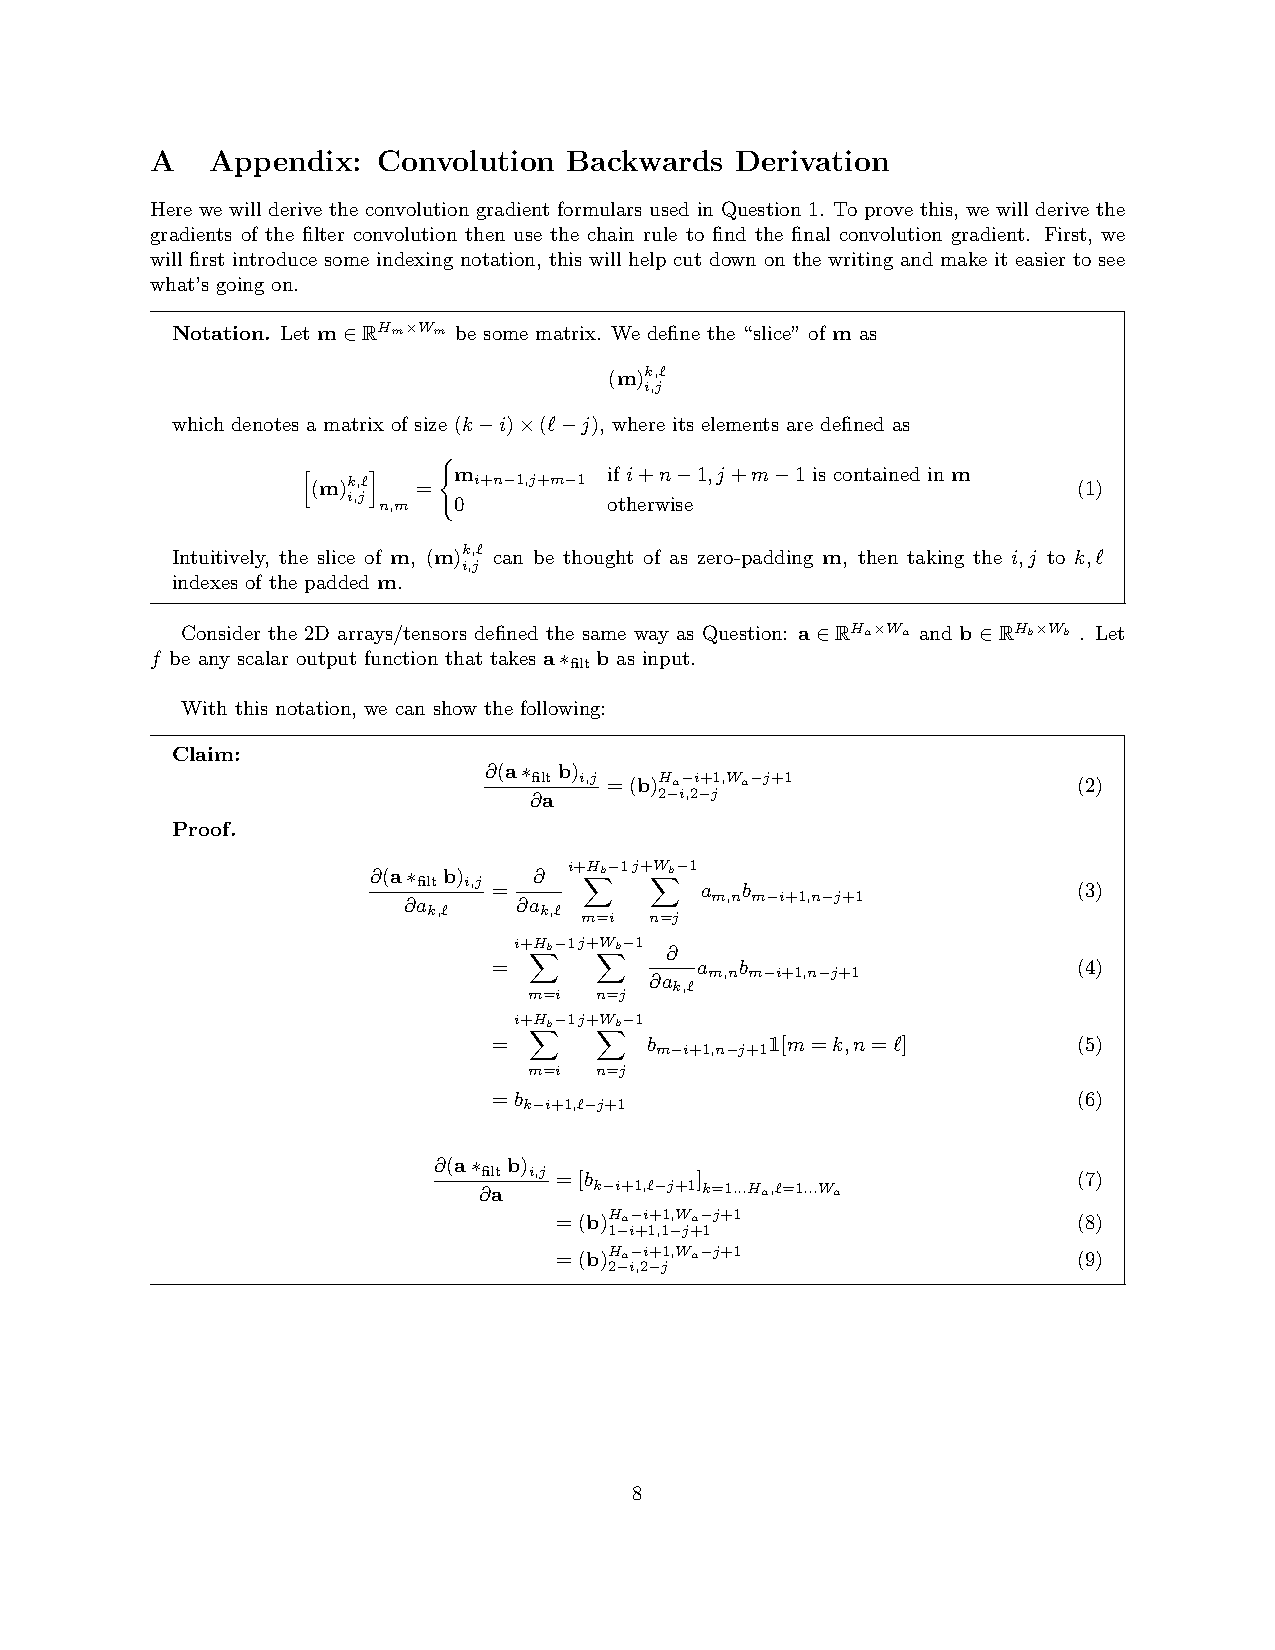
\includepdf[]{hw4_appendix.pdf}







\end{document}